\documentclass[preprint,nocopyrightspace]{sigplanconf}
\usepackage{setspace}
\usepackage{times}
\usepackage{paralist}
\usepackage{amsmath,amssymb,amsfonts}
%%\usepackage{dsfont,pifont}
%%\usepackage{gdefs,graphicx}
%%\usepackage{graph,color}
%\usepackage{changebar}
%\usepackage{subfigure}
\usepackage{subfig}
%\usepackage{proof}
%%\usepackage[sfcode]{ttquot}
%\usepackage{angle}
%\usepackage{code}
%\usepackage{mathpartir}
%\usepackage{ctable}
%\usepackage{verbatim}
%\usepackage{bookmark}
\usepackage[T1]{fontenc}
\usepackage[latin9]{inputenc}
%\usepackage{babel}
\usepackage[dvipsnames,usenames]{color}
\usepackage{float}
\usepackage{graphics}
\usepackage{graphicx}
\usepackage{wrapfig}
\usepackage[ruled,vlined]{algorithm2e}
\usepackage{url}
%\usepackage[pdftex,colorlinks=true, linkcolor=blue,citecolor=blue, urlcolor=blue,bookmarksopen=false]{hyperref}
%\hypersetup{
%  pdfinfo={
%    Title={Abstract Semantic Differencing for Numerical Programs},
%    Author={Partush, Yahav},
%    Keywords={Differential Analysis, Semantic Diff, Patches, Equivalence Checking, Abstract Interpretation, Numerical Domains}
%  }
%}

\usepackage{listings}
\lstset{basicstyle=\ttfamily\scriptsize,emph={},emphstyle={\underbar},numbers=none,escapeinside={(*@}{@*)}}

% Generic macros (nothing specific to this paper)

\usepackage{ifthen}
%
\newcommand{\TODO}[1]{ {\color{blue} \bf #1} }
\newcommand{\AWK}[1]{ {\color{red} \bf #1} }
\newcommand{\TODOFN}[1]{ \footnote{{\bf #1}} }
\newcommand{\DONE}[1]{}
\newcommand{\COMMENT}[1]{}
\newcommand{\ie}{i.e.}
\newcommand{\eg}{e.g.}
%%% references definition
\newcommand{\lemref}[1]{Lemma~\ref{Lm:#1}}
\newcommand{\figref}[1]{Fig.~\ref{Fi:#1}}
\newcommand{\defref}[1]{Definition~\ref{De:#1}}
\newcommand{\theref}[1]{Theorem~\ref{Th:#1}}
\newcommand{\tabref}[1]{Tab.~\ref{Ta:#1}}
\newcommand{\secref}[1]{Section~\ref{Se:#1}}
\newcommand{\secrefs}[2]{Sections~\ref{Se:#1}-\ref{Se:#2}}
\newcommand{\ssecref}[1]{Sec.~\ref{Se:#1}}
%\newcommand{\subref}[1]{Subsection~\ref{Sub:#1}}
\newcommand{\appref}[1]{Appendix~\ref{Se:#1}}
\newcommand{\exref}[1]{Example~\ref{Ex:#1}}
\newcommand{\algref}[1]{Algorithm~\ref{Alg:#1}}
\newcommand{\lnref}[1]{line~\ref{Ln:#1}}
\newcommand{\lemlabel}[1]{\label{Lm:#1}}
\newcommand{\figlabel}[1]{\label{Fi:#1}}
\newcommand{\deflabel}[1]{\label{De:#1}}
\newcommand{\thelabel}[1]{\label{Th:#1}}
\newcommand{\tablabel}[1]{\label{Ta:#1}}
\newcommand{\seclabel}[1]{\label{Se:#1}}
\newcommand{\sseclabel}[1]{\label{Se:#1}}
%\newcommand{\sublabel}[1]{\label{Sub:#1}}
\newcommand{\applabel}[1]{\label{Se:#1}}
\newcommand{\exlabel}[1]{\label{Ex:#1}}
\newcommand{\alglabel}[1]{\label{Alg:#1}}
\newcommand{\lnlabel}[1]{\label{Ln:#1}}


\newtheorem{Example}{Example}
%\newtheorem{definition}{Definition}
%%\newtheorem{theorem}{Theorem}
%%% sectioning

\newcommand{\ignore}[1]{}

%% TO Allow writing the TR in the same source
\newboolean{TR}
\setboolean{TR}{false}
\ifthenelse{\boolean{TR}}{
\newcommand{\TrSelect}[2]{#1}
\newcommand{\TrOnly}[1]{#1}
\newcommand{\SubOnly}[1]{}
\newcommand{\TrOnlyInFootnote}[1]{#1}
\newcommand{\TrOnlyInTable}[1]{#1}}
{
\newcommand{\TrSelect}[2]{#2}
\newcommand{\TrOnly}[1]{}
\newcommand{\SubOnly}[1]{#1}
\newcommand{\TrOnlyInFootnote}[1]{}
\newcommand{\TrOnlyInTable}[1]{}}

%% General macros
\newcommand{\Set}[1]{\{ \; {#1} \; \}}
\newcommand{\vbar}{\; | \;}
\newcommand{\notIn}{\not\in}
\newcommand{\sizeof}[1]{|{#1}|}
%% \newcommand{\isDefined}{=_{def}}
\newcommand{\isDefined}{\triangleq}

\newcommand{\lt}{$<$}
\newcommand{\gt}{$>$}

%% tminus: "thin minus", with less space around it;
%% telem: "thin element"
\newcommand{\tminus}{\!\! - \!\!}
\newcommand{\telem}{\! \in \!}

%% stexttt: "small" texttt
\newcommand{\stexttt}[1]{{\small \texttt{#1}}}

\newcommand{\mathify}[1]{\mathord{\mbox{#1}}}
\newcommand{\italMathId}[1]{\mathify{\textit{\textrm{#1}}}}
\newcommand{\romanMathId}[1]{\mathify{\textup{\textrm{#1}}}}
\newcommand{\ttMathId}[1]{\mathify{\textup{\texttt{#1}}}}

\newcommand{\ttsub}[2]{${\ttMathId{#1}}_{#2}$}
\newcommand{\ttsup}[2]{${\ttMathId{#1}}^{#2}$}
\newcommand{\mttsub}[2]{{\ttMathId{#1}}_{#2}}
\newcommand{\twoarray[2]}{\begin{array}{l}  #1 \\ #2 \end{array}}
\newcommand{\subsubsubsection}[1]{\emph{#1}:}

%\newtheorem{theorem}{Theorem}[section]
%\newtheorem{lemma}[theorem]{Lemma}
%\newtheorem{proposition}[theorem]{Proposition}
%\newtheorem{corollary}[theorem]{Corollary}

%\newenvironment{proof}[1][Proof]{\begin{trivlist}\item[\hskip \labelsep {\bfseries #1}]}{\end{trivlist}}
%\newenvironment{definition}[1][Definition]{\begin{trivlist}\item[\hskip \labelsep {\bfseries #1}]}{\end{trivlist}}
%\newenvironment{example}[1][Example]{\begin{trivlist}\item[\hskip \labelsep {\bfseries #1}]}{\end{trivlist}}
%\newenvironment{remark}[1][Remark]{\begin{trivlist}\item[\hskip \labelsep {\bfseries #1}]}{\end{trivlist}}

%\newcommand{\qed}{\nobreak \ifvmode \relax \else
%      \ifdim\lastskip<1.5em \hskip-\lastskip
%      \hskip1.5em plus0em minus0.5em \fi \nobreak
%      \vrule height0.75em width0.5em depth0.25em\fi}

%% $Id: specificmacros.tex,v 1.22 2010/07/15 18:27:09 mkuper Exp $

\def\imagetop#1{\vtop{\null\hbox{#1}}}

\newcommand{\demonsmarker}{\textbf{DEMONS START HERE IF NOT EARLIER}}

\newcommand{\sectionette}[1]{\noindent \textit{#1}:}

\newtheorem{hypothesis}{Hypothesis}[section]
\newcommand{\hypref}[1]{Hypothesis~\ref{Hy:#1}}

\newcommand{\true}{T}
\newcommand{\false}{F}

\newcommand{\pline}[1]{#1}

\newcommand{\lnum}[1]{\textbf{#1}}
\newcommand{\reflnum}[1]{\texttt{#1}}

\newcommand{\term}[1]{\emph{#1}}

\newcommand{\authortext}[1]{{$\bullet$ \textsf{#1}}}
\newcommand{\hiddentext}[1]{}

\newenvironment{samePageBlock}{\par
\samepage
}{%
\par
\allowbreak }

\newcommand{\para}[1]{\vspace{3pt}\noindent\textbf{\textit{#1}}}
%\newcommand{\Lparagraph}[1]{\vspace{3pt}\noindent\textit{#1.}}
\newcommand{\Lparagraph}[1]{\vspace{-4pt}\paragraph{#1}}
%\newcommand{\LLparagraph}[1]{\noindent\textit{#1.}}
\newcommand{\tab}{\hspace*{2em}}

\newcommand{\correlate}{\bowtie}

\newcommand{\fvar}[2]{[#1\prec #2]}

\newcommand{\better}{\sqsubseteq}
\newcommand{\wbetter}{\unlhd}

\newcommand{\sep}{\ensuremath{\ \ | \ \ }}
\newcommand{\tool}{{\small \textsc{dizy}}}
\newcommand{\fpred}[2]{(#1\prec #2)}
\newcommand{\trans}[3]{#1\stackrel{#3}{\longrightarrow}#2}
\newcommand{\strans}[3]{#1\longrightarrow#2}
\newcommand{\mmname}{{\small \textsc{RLX}}}
\newcommand{\ebset}{\hat{E}}

\newcommand{\B}[1]{\langle{#1}\rangle}
\newcommand{\eqdef}{\buildrel \mbox{\tiny\rm def} \over =}

%%%%%%%%%%%%%%%%%%%%%%%%%%%%%%%%%%%%%%%%%%%%%%%%%%%%%
%% notation                                        %%
%%%%%%%%%%%%%%%%%%%%%%%%%%%%%%%%%%%%%%%%%%%%%%%%%%%%%

\newcommand{\optimal}{\ding{52}}
\newcommand{\success}{\ding{51}}
\newcommand{\failure}{\ding{55}}

%%%%%%%%%%%%%%%%%%%%%%%%%%%%%%%%%%%%%%%%%%%%%%%%%%%%%
%% Abstraction                                     %%
%%%%%%%%%%%%%%%%%%%%%%%%%%%%%%%%%%%%%%%%%%%%%%%%%%%%%

\newcommand{\eq}[1]{[#1]_{\alpha}}%{eq(#1)}

%%%%%%%%%%%%%%%%%%%%%%%%%%%%%%%%%%%%%%%%%%%%%%%%%%%%%
%% Terminology                                     %%
%%%%%%%%%%%%%%%%%%%%%%%%%%%%%%%%%%%%%%%%%%%%%%%%%%%%%
\newcommand{\scode}[1]{{\small \texttt{#1}}}
\newcommand{\sname}[1]{{\small \textsc{#1}}}

%%%%%%%%%%%%%%%%%%%%%%%%%%%%%%%%%%%%%%%%%%%%%%%%%%%%%
%% Actions and Traces                              %%
%%%%%%%%%%%%%%%%%%%%%%%%%%%%%%%%%%%%%%%%%%%%%%%%%%%%%

\newcommand{\interseq}[1]{{\small\texttt{#1}}}

%%%%%%%%%%%%%%%%%%%%%%%%%%%%%%%%%%%%%%%%%%%%%%%%%%%%%
%% Semantics                                       %%
%%%%%%%%%%%%%%%%%%%%%%%%%%%%%%%%%%%%%%%%%%%%%%%%%%%%%

\newcommand{\lsyn}{\lbrack\!\lbrack}
\newcommand{\rsyn}{\rbrack\!\rbrack}
\newcommand{\semp}[1]{\lsyn #1 \rsyn}
\newcommand{\asemp}[1]{\lsyn #1 \rsyn^{\sharp}}

\newcommand{\slen}[1]{|#1|}

\newcommand{\dpless}{<_{\sigma,p}}

\newcommand{\concat}{\cdot}

%% States
\newcommand{\States}{\Sigma}
\newcommand{\sStates}{\Sigma_s}
\newcommand{\pStates}{\Sigma_p}
\newcommand{\mStates}{\Sigma_M}

%% Transitions
\newcommand{\Transitions}{\mbox{{\it \Tau}}}
\newcommand{\pTrans}{\Tau_p}
\newcommand{\mTrans}{\Tau_M}


%% Sets of States
\newcommand{\Stuck}{\mbox{{\it Stuck}}}
\newcommand{\Doomed}{\mbox{{\it Doomed}}}
\newcommand{\Initial}{\mbox{{\it Init}}}


%% Program
\newcommand{\Labels}{\italMathId{Labs}}
\newcommand{\Statements}{\italMathId{Stmts}}
\newcommand{\SharedVar}{\italMathId{Shared}}
\newcommand{\LocalVar}{\italMathId{Local}}
\newcommand{\stmt}{\mbox{{\it stmt}}}
\newcommand{\Value}{\mbox{{\it Int}}}
\newcommand{\val}[2]{\semp{#1}(#2)}
\newcommand{\Reach}{\mbox{{\it Reach}}}

%% Relations
\newcommand{\patharrow}{\rightsquigarrow}

%% General
\newcommand{\valid}{\mbox{{\it valid}}}
%\newcommand{\implies}{\Rightarrow}
\newcommand{\wgamma}{\widehat{\gamma}}
\newcommand{\powerset}{\mathcal{P}}
\newcommand{\dominatedBy}{\mbox{{\it DominatedBy}}}
\newcommand{\Ideal}{\mbox{{\it Ideal}}}
%\newcommand{\Obs}{\mbox{{\it Obs}}}
\newcommand{\Op}{\mbox{{\it Op}}} %% operations
\renewcommand{\phi}{\varphi}


\newcommand{\atomic}[2]{{\footnotesize \texttt{[#1,#2]}}}

\newcommand{\atomicmath}[2]{[#1,#2]}

\newcommand{\scheduled}{\mbox{\textit{atomic}}}
\newcommand{\nodes}{\mbox{\textit{states}}}

\newcommand{\MA}{\mbox{\textit{MA}}}

\newcommand{\aeq}{\preceq_{\alpha}}

\newcommand{\Abs}{\Sigma^{\natural}_P}
\newcommand{\Traces}{\mbox{\scode{Traces}}}

\newcommand{\C}[1]{#1^\natural} % for all concrete symbols
\newcommand{\A}[1]{#1^\sharp} % for all abstract symbols
\newcommand{\PS}[1]{{2^{#1}}}
\newcommand{\StatesConc}{\C{C}}
\newcommand{\Formulas}{Formulas}
\newcommand{\Dom}{Dom}
\newcommand{\Below}{\sqsubseteq}
\newcommand{\violated}{Av}
\newcommand{\UStates}{\Upsilon}
\newcommand{\evalf}[2]{\llbracket #2 \rrbracket_{#1}}
\newcommand{\enf}[2]{E_{\fpred{#1}{#2}}}
\newcommand{\admits}[2]{#1\smile #2}
\newcommand{\nadmits}[2]{#1\not\smile #2}

\newcommand \abssem[1]{Abs\textsubscript{[1,#1]}}
\newcommand{\semref}[1]{Sem.~\ref{Fi:#1}}

%\newcommand{\SBa}{SB1}
\newcommand{\SBb}{RA}
\newcommand{\SBc}{PDA}
\newcommand{\SBd}{OA}

\newcommand{\NoPJ}{FD}
\newcommand{\PJ}{PD}

\newcommand{\PD}[1]{{#1}^\tau}


\begin{document}

\title{Abstract Semantic Differencing for Numerical Programs}

\authorinfo{Nimrod Partush}{Technion}{nimi@cs.technion.ac.il}
\authorinfo{Eran Yahav}{Technion}{yahave@cs.technion.ac.il}

\maketitle

\begin{abstract}
We address the problem of correlating closely related versions of a program.
\end{abstract}


\section{Introduction} \seclabel{Intro}

%% what are we trying to say?
% 1. computing semantic diff is important
% 2. computing semantic diff is hard
% 3. existing approaches for computing semantic diff suck
% 4. our approach is great
% 5. technically, we use the following ideas:
%    - correlating program
%    - correlating abstract domains

% TODO:
% - we should have a clear problem definition somewhere
% - what is so special about a patched program?

Understanding the semantic difference between two versions of a program is invaluable in the process of software development. A developer applying a patch is often interested in answering questions like:
\begin{inparaenum}[(i)]
\item did the patch add/remove the desired functionality?
\item does the patch introduce other, \emph{unexpected}, behaviors?
\item which regression tests should be run?
\end{inparaenum}
Answering these questions manually is difficult and time consuming.

Semantic differencing has received much attention in classical work (e.g.,~\cite{Horwitz90,Horwitz89,Hoare69}) and has recently seen growing interest for various applications ranging from testing of concurrent programs~\cite{ChakiGurfinkelStrichman12}, understanding software upgrades~\cite{JinOrsoXie10}, to automatic generation of security exploits~\cite{BrumleyPoosankamSongZheng08}.

\para{Problem Definition}
We define the problem of \emph{semantic differencing} as follows: Given a pair of programs $(P,P')$ that agree on the number and type of input and output variables, for every execution $\pi$ of $P$ that originates from an input $i$ and a corresponding execution $\pi'$ of $P'$ that originates from the \emph{same input $i$} our goal is:
\begin{itemize}
\item Check whether $\pi$ and $\pi'$ have the same output i.e. are output-equivalent.
\item In case of difference in output variables, provide a description of the difference.
\end{itemize}

\para{Existing Techniques}
Existing techniques mostly offer solutions based on  under-approximation, the most prominent of which is regression testing which provides limited assurance of behavior equivalence while consuming significant time and compute resources. \COMMENT{Kawaguchi et al.~\cite{KawaguchiLahiriRebelo10} define the notion of conditional equivalence but cannot compute differences in loops.}
Other approaches for computing semantics differences~\cite{DwyerElbaumPerson08,EnglerRamos11} rely on symbolic execution techniques, may miss differences, and are generally unable to prove equivalence. Previous work for equivalence checking~\cite{GodlinStrichman09} rely on unsound bounded model checking techniques to prove (input-output) equivalence of two closely related numerical programs, under certain conditions (see \secref{Related} for more details).

\para{Our Approach}
We present an approach based on abstract interpretation~\cite{CousotCousot77} for producing a \emph{sound} representation of changed program behaviors and proving equivalence between a program and a patched version of the program. Our method focuses on abstracting relationships between variables in both versions allowing us to achieve a precise description of the difference and prove equivalence. Our solution is sound in the sense that it computes an over approximation of the difference between the two versions, therefore guaranteeing equivalence when no difference is found.

We focus on output equivalence in the final state. This is sufficient as mid-execution output can be modeled as added variables in the final state. This limitation also means that we assume all program executions to be finite (i.e. equivalence/difference holds if indeed both executions terminate). Note that the definition limits program difference to the final state which alleviates the need for matching the different stages of $(P,P')$. Finding equivalence/difference in earlier stages of the program requires program matching (we first need to find a suitable location in both programs for checking for equivalence, otherwise it has no meaning). The problem of program matching is orthogonal and can be addressed via various techniques ranging in complexity and precision - from syntactic diff~\cite{HuntMcIlroy75} to execution indexing~\cite{Xin:2008} and others. In this work we employ a simple matching strategy to achieve better precision as described in \secref{Correlating}. We found this technique to be sufficient for our experiments.

To answer the question of semantic differencing for infinite-state programs, we employ abstract interpretation. Though the notion of difference is well defined in the concrete case, defining and soundly computing it under abstraction is challenging:
\begin{itemize}
\item Differencing requires correlation of \emph{different program executions}. The abstraction must be able to capture and compare only the input-equivalent executions, and avoid comparing ones that are not input-equivalent.
\item Equivalence of abstract output values does not entail concrete value equivalence.
\end{itemize}

To address these challenges, we introduce two new concepts:
\begin{inparaenum}[(i)]
\item \emph{correlating program} - a single program $P \correlate P'$ that captures the behaviors of both $P$ and $P'$ in a way that facilitates abstract interpretation;
\item \emph{correlating abstract domain} - a domain for tracking relationships between variables in $P$ and variables in $P'$ using $P \correlate P'$.
\end{inparaenum}

\para{Correlating Program}
We create a single program which captures the behavior of both the original program and its patched version. A \emph{correlating program} $P \correlate P'$ contains both programs flow and data, however program flow is arranged so to reflect a (simple) matching between the stages of the two programs. This matching is key for precision as otherwise we will not be able to maintain equivalence throughout the entire run of the program, particularly in the face of loops.

\para{Correlating Abstraction}
Abstracting relationships allows us to maintain focus on differences while over-approximating (whenever necessary for scalability) equivalent behaviors. We abstract variables of both programs together, starting off by assuming equality over all matched variables (variable matching is discussed in \secref{ConcreteSem}). Thus we can
reflect relationships without necessarily knowing the actual value of
variables. We focus on numerical programs and use numerical domains such as Octagon~\cite{Mine2006} and Polyhedra~\cite{CousotHalbwachs78} to capture the relationship between variables. Our current implementation does not track pointer equivalences, but such equivalences can be tracked by a using a correlating shape analysis domain~\cite{AmitRinetzkyRepsSagivYahav07}. To maintain equivalence as much as possible, our domain was designed to represent non-convex information (e.g. so we will not immediately lose equivalence taking a condition of the form $x \neq 0$ into account). We use a powerset domain of convex sub-states. Our domain uses a partitioning strategy that abstracts together states that have the same set of equivalent variables, thus avoiding exponential blowup (as explained in \secref{AbstractSem}). This strategy helps use preserve equivalence even across widening. Therefore our domain may over-approximate numerical information as long as equivalence between correlated variables is preserved.

\subsection{Main Contributions}
The main contributions of this paper are as follows:
\begin{itemize}
\item We present a novel approach for computing abstract semantic difference between a program $P$ and a patched version of the program $P'$. We focus on numerical programs where the values of variables have no a-priori bounds.
\item We reduce the problem of analyzing the two programs $P,P'$ to the problem of analyzing a single \emph{correlating program} $P \correlate P'$ that captures the behavior of $P$ and $P'$.
\item We present a \emph{correlating abstract domain} that captures an over-approximation of the difference between P and P' by tracking relationships between variables in $P \correlate P'$. The domain applies a partitioning strategy for scaling the analysis while maintaining precision in equivalence.
\item We have implemented our approach in a tool based on the \sname{LLVM} compiler infrastructure and the \sname{APRON} numerical abstract domain library, and applied it to several real-world programs. Our evaluation shows that the tool often manages to establish equivalence, reports useful approximation of semantic differences when differences exists, and reports only a few false differences.
\end{itemize}

\section{Overview}\seclabel{Overview}

\begin{figure}
\centering
\begin{tabular}{ccc}
\begin{lstlisting}
int sign(int x) { 
  int sgn;
  if (x < 0)
    sgn = -1
  else 
    sgn = 1
 return sgn
}
(*@ \vspace{0.1in} @*)
\end{lstlisting}
&
&
\begin{lstlisting}
int sign'(int x) {
  int sgn;
  if (x < 0)
    sgn = -1
  else if (x==0)
    sgn = 0
  else 
    sgn = 1
 return sgn
}
\end{lstlisting}
\\
\end{tabular}
\caption{Two simple implementations of the \emph{sign} operation.}
\figlabel{SignExample}
\end{figure}


Consider the simple example program of~\figref{SignExample}, inspired by an example from~\cite{MauborgneRival07}. For this example, we would like to establish that the output of $sign$ and $sign'$ only differ in the case where $x=0$ and that the difference is $sgn = 1 \neq sgn' = 0$. An optimal characterization of behavior is as following:
\\
\begin{tabular}{l|l|l}
$x.x'$ constraints  & $sgn$             & $sgn'$
\\ \hline
$x < 0$             & $sgn \mapsto -1$  & $sgn' \mapsto -1$
\\ \hline
$x = 0$             & $sgn \mapsto 1$  & $sgn' \mapsto 0$
\\ \hline
$x > 0$             & $sgn \mapsto 1$  & $sgn' \mapsto 1$
\end{tabular}
\\

As a first naive attempt to achieve such a description, one could try to analyze each version of the program separately and compare the (abstract) results. However, this is clearly unsound, as equivalence under abstraction does not entail concrete equivalence. For example, using a interval analysis~\cite{CousotHalbwachs78} would yield that in both programs the value of \scode{sgn} ranges in the same interval $[-1,1]$, missing the fact that $sign$ never returns the value $0$.

%\begin{wrapfigure}{r}{0cm}
%\imagetop{
%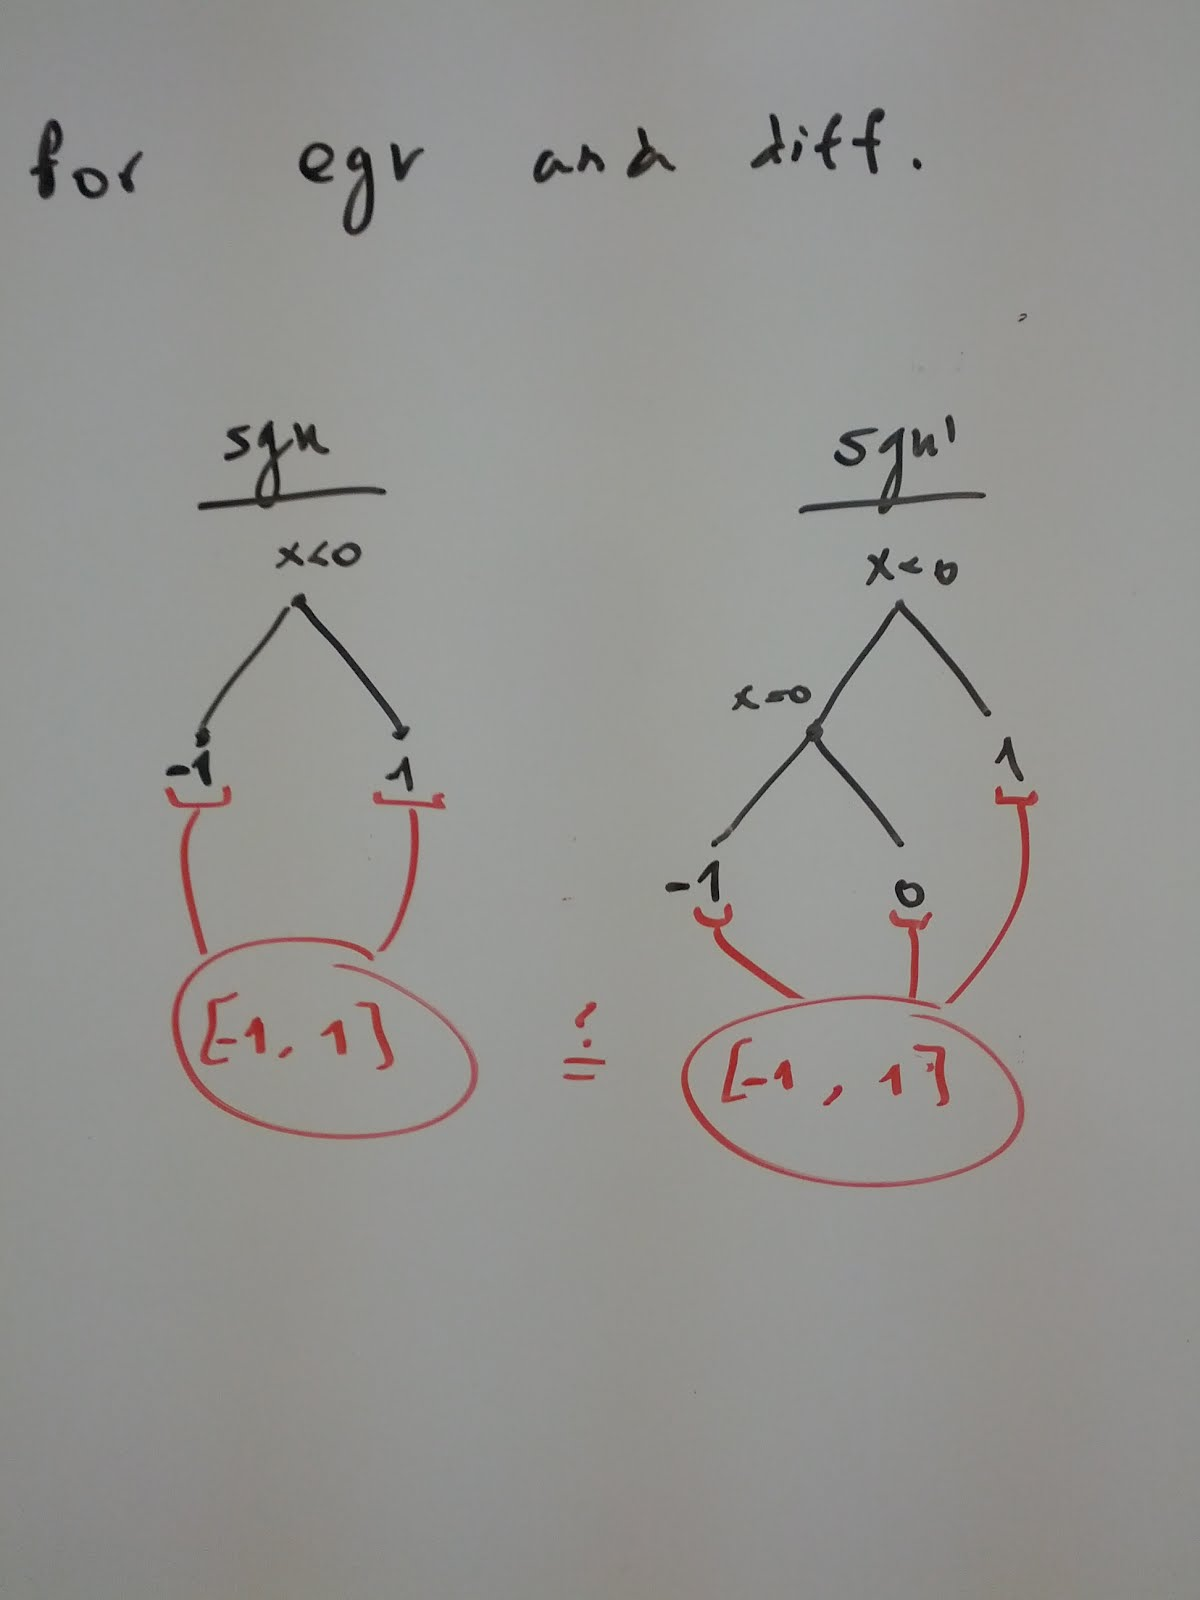
\includegraphics[scale=0.15,clip=true,trim = 125pt 400pt 125pt 350pt]{figures/sign-interval.jpg}
%}
%\caption{Interval analysis unsound comparison for $sign$ and $sign'$}\figlabel{SignInterval}
%\end{wrapfigure}

Furthermore, this result entirely ignores how $x$ affects the value of $sgn$ thus we would have no means to differentiate correctly, by input (e.g. we will get the same result for the $-1 * sign$ function).

To establish equivalence under abstraction, we need to abstract relationships between the values of variables in $sign$ and $sign'$ under the assumption of equivalence of input. Specifically, we need to track the relationship between the values of \scode{sgn} in both versions and see whether we can establish their equivalence. Tracking relationships dictates performing a \emph{joint analysis} that employs a \emph{correlating abstraction} allowing us to bind variables of both programs in one abstract state.

A correlating-oriented abstraction is well suited for proving equivalence as it allows focusing on relationships between versions of variables while abstracting away other (numerical) information allowing us to scale better. Most importantly, such an abstraction guarantees that equivalence will be reported soundly: as in a separate analysis we abstracted $\langle sgn \mapsto -1 \rangle$ and $\langle sgn \mapsto 1 \rangle$ towards an interval $\langle sgn \mapsto [-1,1] \rangle$, and again for $sgn'$ values, separately, which cannot assure equivalence (and in fact shouldn't). We instead use correlating states: $s_1 = \langle sgn = sgn' \mapsto -1 \rangle$ and $s_2 = \langle sgn = sgn' \mapsto 1 \rangle$, which allow us to abstract as such $s_1 \sqcup s_2 = \langle sgn = sgn', sgn \mapsto [-1,1] \rangle$ so equivalence can be soundly assured.

%If we instead use disjunctive completion powerset domain~\cite{TODO} where the abstract state is a set of convex sub-states, and no merge is ever performed, this would yield a precise result that may be used for equivalence checking and differencing.  For instance, using such domain for $sign$ would yield: $\langle x < 0, sgn = -1 \rangle \vee \langle x \geq 0, sgn = 1 \rangle$ and for $sign'$: $\langle x < 0, sgn = -1 \rangle \vee \langle x > 0, sgn = 1 \rangle \vee \langle x = 0, sgn = 0 \rangle$. Further refining $sign$'s abstraction and splitting the $\langle x \geq 0, sgn = 1 \rangle$ constraint to $\langle x > 0, sgn = 1 \rangle \vee \langle x = 0, sgn = 0 \rangle$ would allow perfectly aligning the input constraints to produce the difference of $x=0,sgn=1,sgn'=0$ as depicted in \figref{SignComplete}.
%\begin{wrapfigure}{r}{0cm}
%\imagetop{
%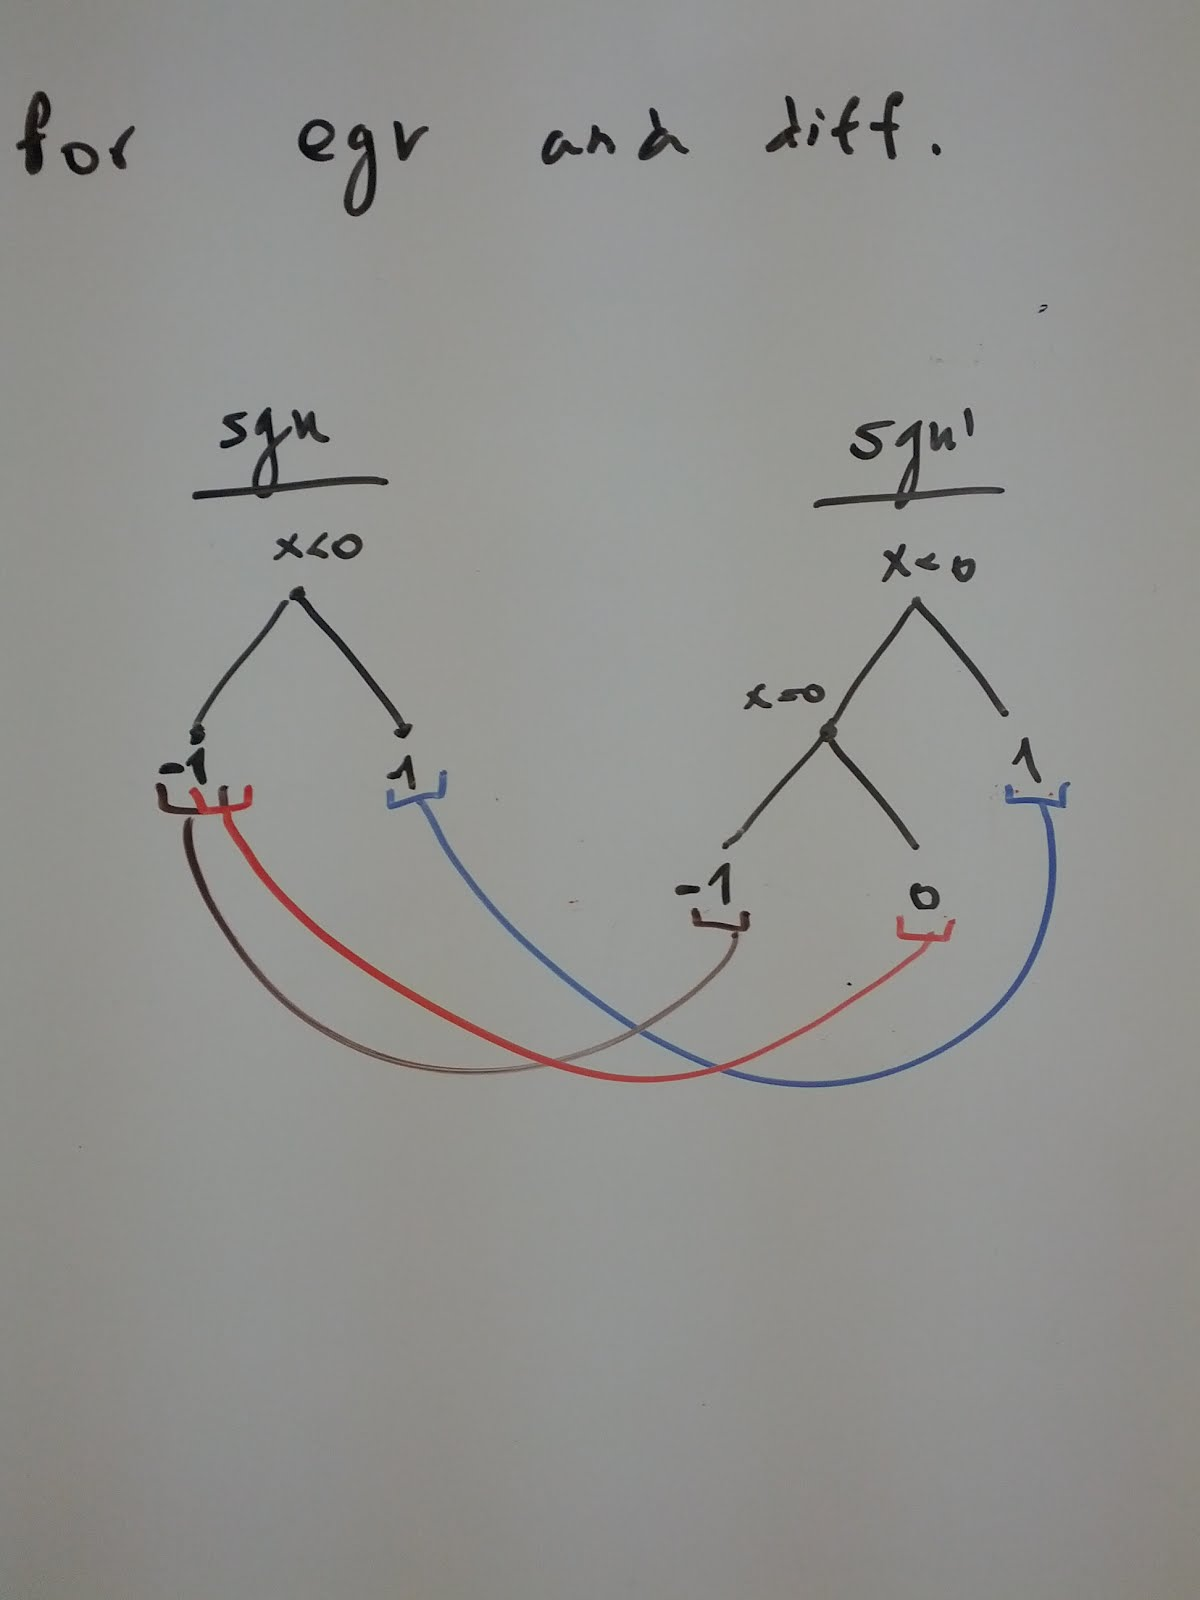
\includegraphics[scale=0.15,clip=true,trim = 125pt 450pt 100pt 350pt]{figures/sign-complete.jpg}
%}
%\caption{Complete disjunction analysis sound comparison for $sign$ and $sign'$}\figlabel{SignComplete}
%\end{wrapfigure}

We present an abstraction over dual program state, thats able to correlate paths that originate from the same input as well as produce a characterization of equivalence and difference which reflects change in behavior precisely. For example, we produce the following constraints for $sign$ and $sign'$:
\\
\begin{tabular}{ccc}
\hspace{1cm} $\sigma_{\times}^1 = \{x = x' < 0, sgn = sgn' \mapsto -1\}$
\\
\hspace{1cm} $\sigma_{\times}^2 = \{x = x' = 0, sgn \mapsto 1, sgn' \mapsto -1\}$
\\
\hspace{1cm} $\sigma_{\times}^3 = \{x = x' > 0, sgn = sgn' \mapsto 1\}$
\\
\end{tabular}
\\

To arrive at this result, we used an initial setting which abstracted the dual program state by analyzing both programs sequentially ($P;P'$), while updating the shared state with data regarding both sets of variables, while allowing a complete disjunction over all paths. In order to correlate paths by input and arrive at a precise disjunction, the analysis initially assumes input equivalence $\vec{i} = \vec{i'}$.

In this setting, as we advance through the analysis of $P$, we will accumulate the disjunction of all possible path constraints in its final state (this is similar to trace partitioning~\cite{MauborgneRival07}). At this point, as we continue to analyze $P'$, each disjunct representing a path in $P$ will be further conjuncted with all of $P'$ paths. This will produce a precise disjunction for differencing as each path in $P$ will be split and conjuncted with all of $P'$ paths, while avoiding considering conjunctions that disagree on input due to our input equivalence assumption. An illustration of the joint analysis for the $sign$ example can be seen in \figref{SignAnalysis1} including markings for feasible and infeasible paths.

%In some cases, it would have been sufficient to use alternative domains that are capable of representing richer information, such as interval polyhedra~\cite{CMWC:SAS09}, or other numerical domains that can represent non-convex information (e.g., \cite{TODO}). The recent donut domain~\cite{GIBMG:VMCAI12} may be of particular interest for this purpose. However, the general principle of having to preserve correlating information even when information about the values is abstracted away, holds in all of these cases.

%\begin{figure}
%\imagetop{
%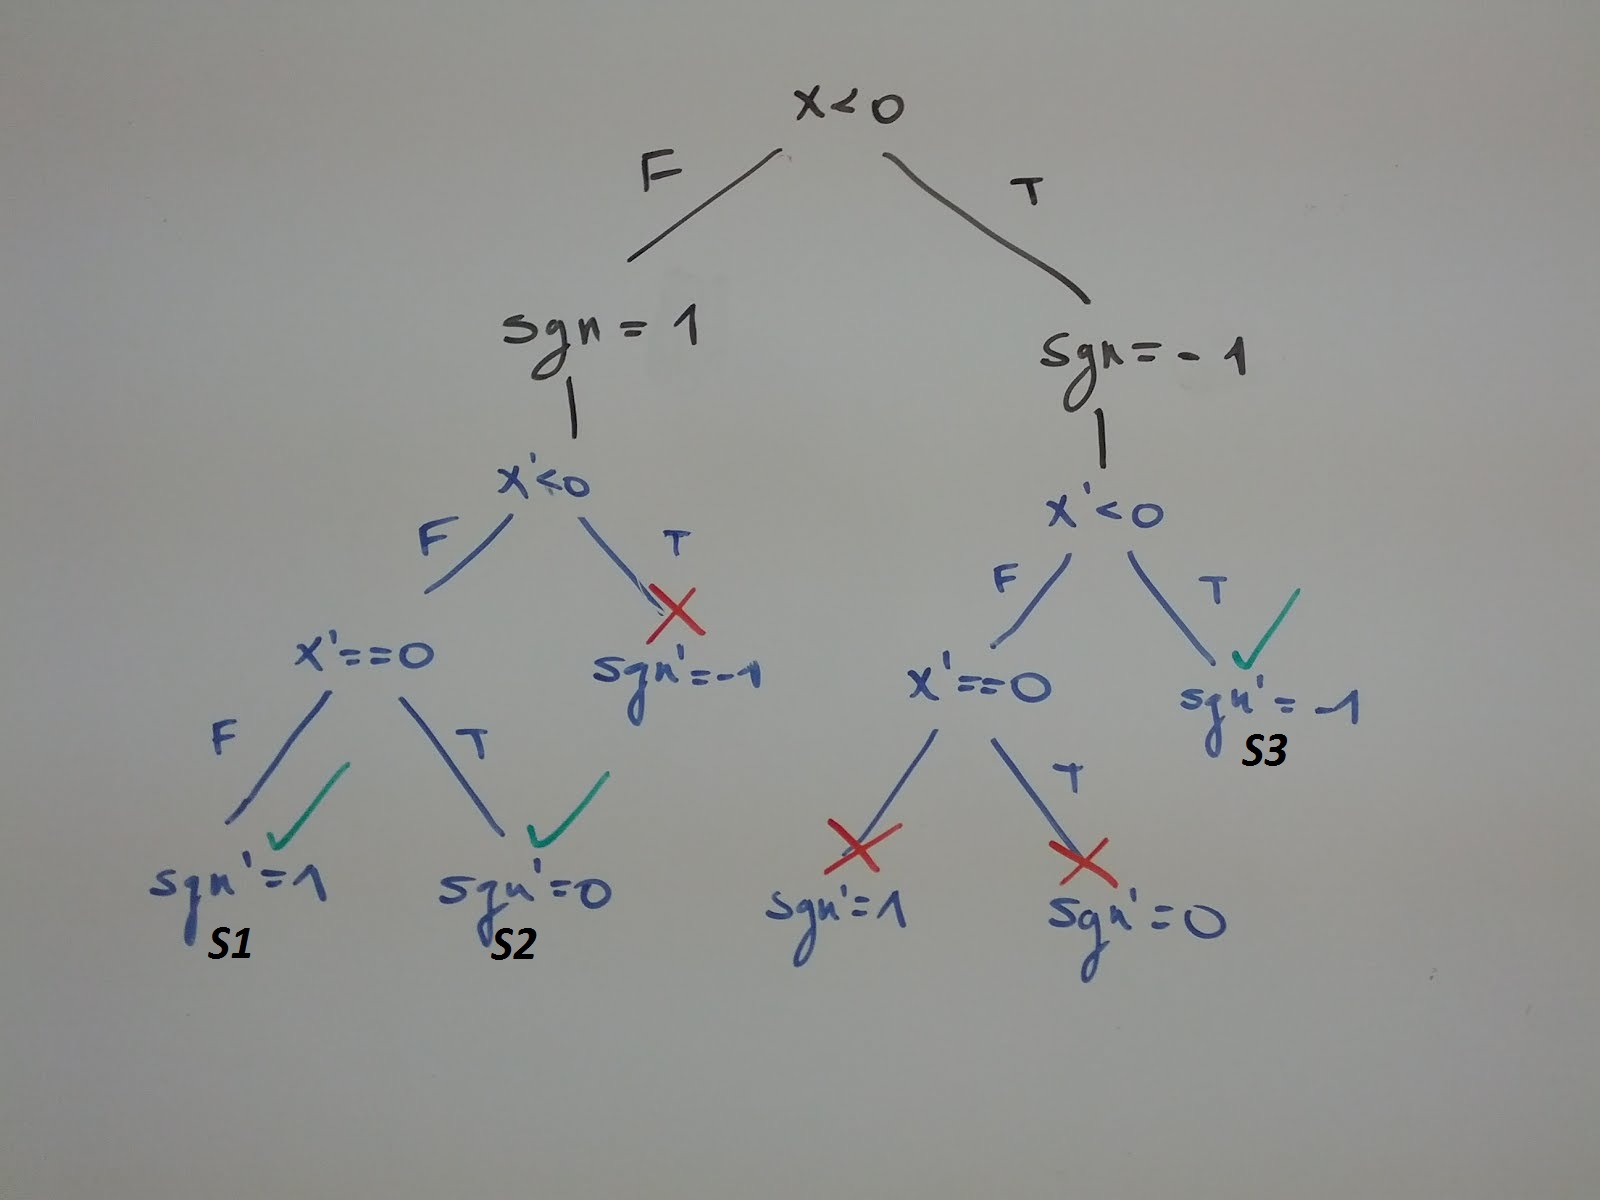
\includegraphics[scale=0.28,clip=true,trim = 50pt 100pt 100pt 0pt]{figures/sign-analysis1.jpg}
%}
%\caption{Joint $sign;sign'$ analysis}\figlabel{SignAnalysis1}
%\end{figure}

\begin{figure}
\centering
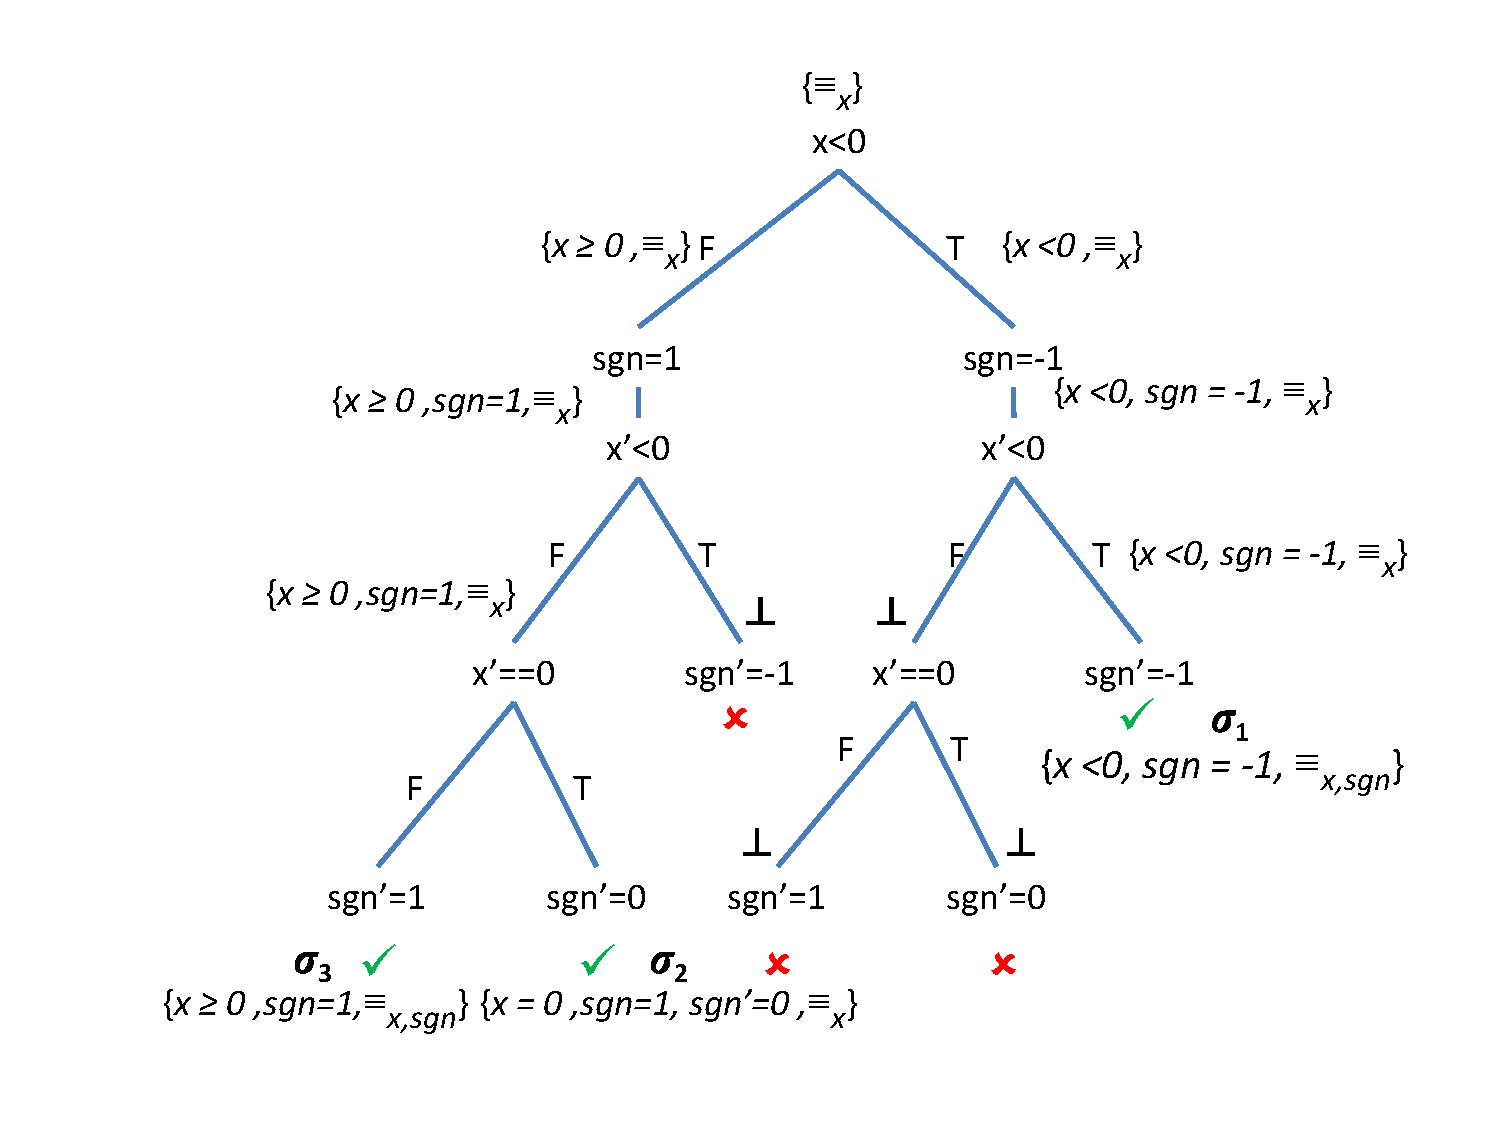
\includegraphics[scale=0.38,clip=true,trim = 75pt 25pt 5pt 20pt]{figures/sign-graph-joint}
\caption{Joint $sign;sign'$ analysis}\figlabel{SignAnalysis1}
\end{figure}

Essentially, our analysis aims to establish correspondence between paths in $P$ and $P'$ by first analyzing all of $P$ paths and then attempting to correlate with $P'$ paths. Clearly, this abstraction is unfeasible for most cases as the number of paths to be considered is exponential (we defer the case of loops where this number is unbound). Therefore we refine our abstraction by using a partially disjunctive domain, partitioned by \emph{equivalence criteria}.

%However, analyzing over $P;P'$ means in the worst case remembering the states along each $P$-path and relating them to states in the corresponding $P'$-path. This approach is similar to the symbolic execution approach~\cite{} where all possible correlating paths are explored individually and output is examined to determine difference whilst attempting to reach full coverage. Much like this approach, this abstraction is unfeasible for most cases, especially for programs with an unbound number of paths e.g. \textbf{loops}. To avoid this we move to a partially disjunctive domain, partitioned by \emph{equivalence criteria}.

As the goal of work is to distinguish equivalent from differencing behaviors, using equivalence as criteria for merging paths is apt. The partitioning will abstract together paths that hold equivalence for the same set of variables, allowing for a maximum of $2^{|VC|}$ disjunctions in the abstract state, where $VC$ is the set of correlated variables. So far we have implicitly defined $VC$ as a correlation between $P,P'$ input and outputs, but our approach is in fact parameterized by this matching, allowing for any $P$ variable to be matched with any of $P'$ which has the potential to provide a more precise result (in the cost of scaling) or alternatively provide a more coarse, scalable result by allowing less variables or only certain equivalence classes of $2^{VC}$. A formal definition and discussion of $VC$ is found in \secref{ConcreteSem}.

For example partitioning the result of \figref{SignAnalysis1} according to our criteria would abstract behaviors $s_1$ and $s_3$ together, as they hold equivalence for $sgn$. The merge would abstract away data regarding $x$ and represent $sgn$ as the $[-1,1]$ interval, losing precision but gaining reduction in state size. This lose of precision is acceptable as it is complemented by the offending state $s_2$. Still, not much is gained from this partitioning, as it is performed at the final state, where we may have already reached an exponential amount of disjunctions.

\begin{figure}
\centering
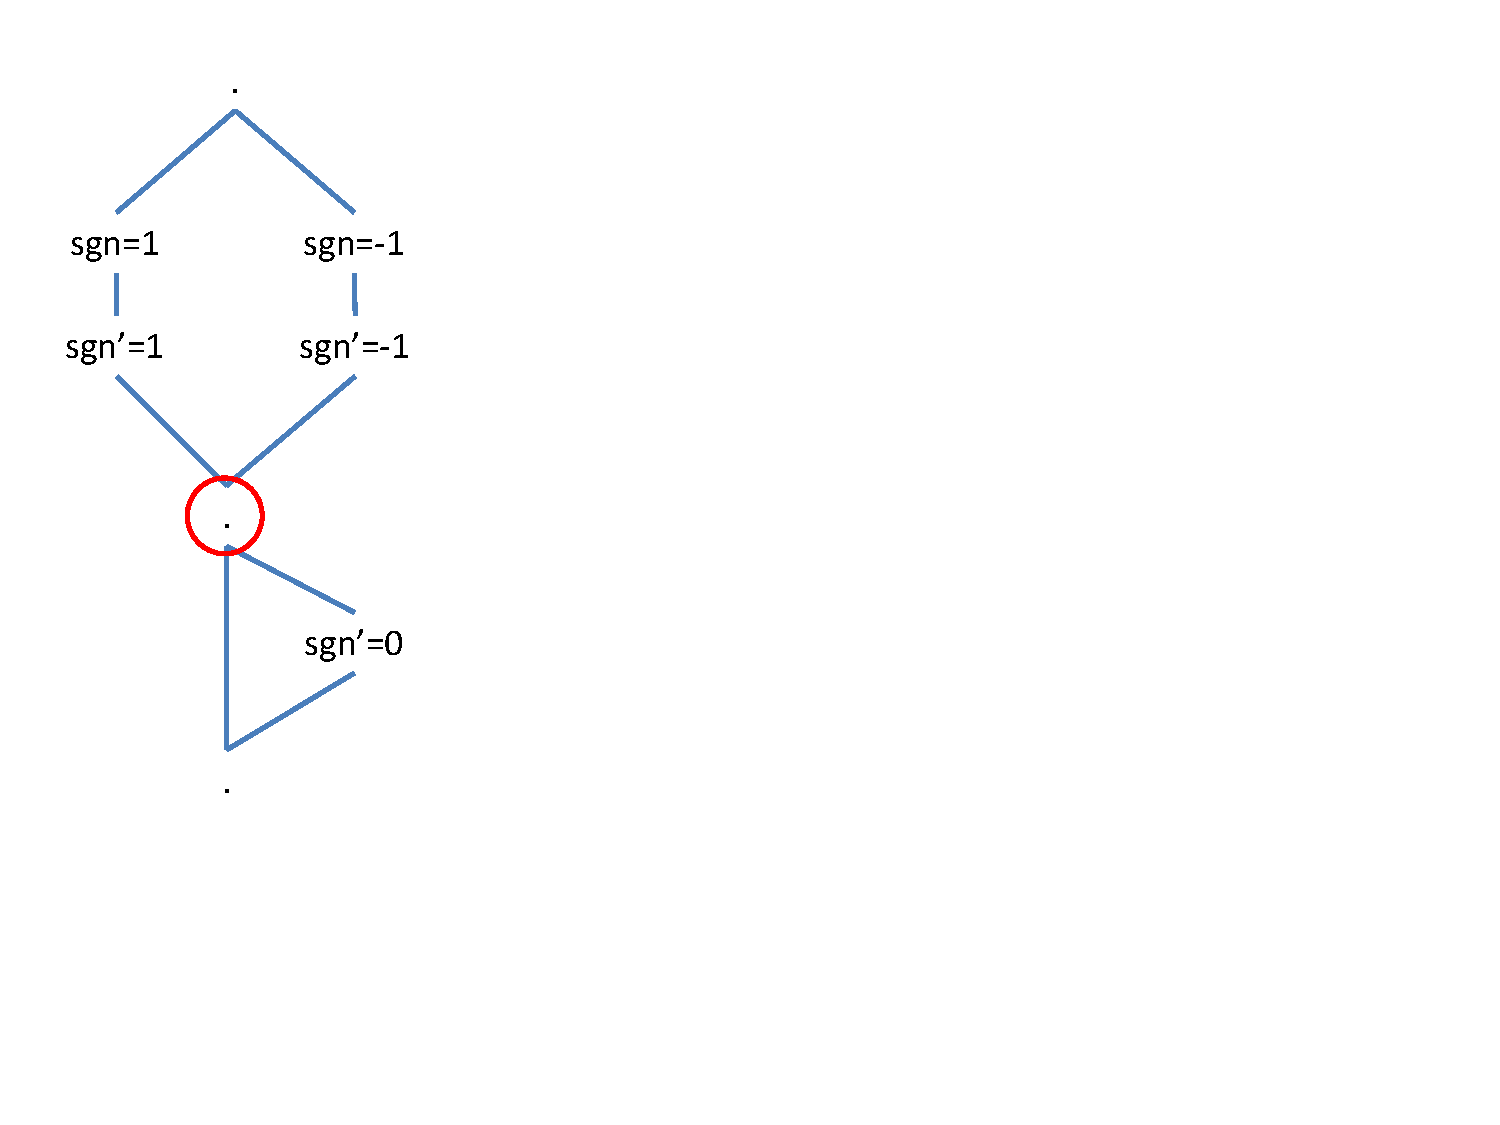
\includegraphics[scale=0.42,clip=true,trim = 0pt 150pt 450pt 150pt]{figures/sign-graph-correlated}
\caption{$sign \bowtie sign'$ analysis}\figlabel{SignAnalysis2}
\end{figure}

To truly gain a reduction of state size, we must perform partitioning dynamically as the analysis is executed i.e. at earlier program locations. This cannot be achieved using a sequential composition $P;P'$. Looking at \figref{SignAnalysis1} we immediately see that equivalence holds only at final states. Intuitively, this is caused due to a command in $P$ having to "wait" for its equivalent command to arrive in $P'$. To overcome this, we present the correlating program $P \bowtie P'$ which allows for earlier partitioning by "saving the need to wait". $P \bowtie P'$ interleaves $P$ and $P'$ commands in an optimized manner, and informs the analysis that it need not wait any further and partitioning is permitted. \figref{SignAnalysis2} depicts the analysis of $sign \bowtie sign'$ (shown in \figref{SignCorrelating}) where the partitioning location is marked with a circle. We define these partitioning locations as \emph{correlation points} (denoted $CP$) and they are a sub product of the correlating program build process. We will further describe the specifics of creating $P \bowtie P'$ in \secref{Correlating} and only shortly say that the interleaving is chosen according to a syntactic diff process over a guarded command language version of the programs.

\begin{figure}
\centering
\begin{lstlisting}
// Nimrod - please fill this 
\end{lstlisting}
\caption{Correlating program $sign \correlate sign'$.}
\figlabel{SignCorrelating}
\end{figure}


% bite the bullet and do widening.
Although we achieved a reduction in state size using partitioning, we have yet to account for programs with an unbound number of paths, created by loops. Unbound path lengths means a potentially unbound analysis as all paths are abstracted. This is mainly where previous approaches fall short ~\cite{GodlinStrichman09, KawaguchiLahiriRebelo10, DwyerElbaumPerson08, EnglerRamos11}. To overcome this, we define a widening operator for our domain, based on the convex sub-domain widening operator. The main challenge here, as our state is a set of convex objects, is finding an optimal pairwise matching between objects for a precise widened result. Optimally, we would like to pair objects that adhere to the same "looping path" meaning we would want to match a path $\pi_i$'s abstraction with a path $\pi_{i+1}$ that results from taking another step in the loop. This basically requires encoding path information along with the sub-state abstraction. This information is acquired by simply keeping guard values explicitly, as they appear in our correlating program, inside the state. As guard values (true or false) reflect branch outcomes, they can be used to match sub-states that advanced on the loop by matching their guard values (for easier matching and better precision we separate guards from other variables in our implementation).

\begin{figure}
\centering
\begin{lstlisting}
int sum(int arr[], unsigned len) {
  int result = 0;
  for (unsigned i = 0; i < len; i++)
    result += arr[i];
 return result;
}
\end{lstlisting}
\caption{A simple looping program for array summation.}
\figlabel{LoopExample}
\end{figure}

We note that the correlating program is cruicial to maintaining equivalence over loops. To demonstrate this we perform the simple exercise of checking equivalence of a small looping program with itself. Consider the array summation program in \figref{LoopExample}. Equivalence for these two small programs cannot be established soundly by approached based on under approximation. To emphasize the importance of the correlating program, we will first show the result of an analysis of $sum;sum'$ which will be:
\\
\begin{tabular}{c}
\hspace{1cm} $\sigma_{\times}^1 = \{len = len' \leq 1, result = result' \mapsto 0\}$
\\
\hspace{1cm} $\sigma_{\times}^2 = \{len = len' > 1\}$
\end{tabular}
\\
\begin{figure}
\centering
\begin{lstlisting}
int sum(int arr[], unsigned len) {
  unsigned len' = len;
  int arr'[] = arr;
  int result = 0;
  int result' = 0;
  {
    unsigned i = 0;
    unsinged i' = 0;
l:  guard g = (i < len);
l': guard g' = (i' < len');
    if (g) result += arr[i];
    if (g') result' += arr'[i'];
    if (g) i++;
    if (g') i'++;
    if (g) goto l;
    if (g') goto l';
  }
}
\end{lstlisting}
\caption{$sum \bowtie sum$}
\figlabel{LoopExample}
\end{figure} 
This lose of equivalence occurred due to the inability precisely track the relationship of $result$ and $result'$ over $sum;sum'$. As we widened the first loop to converge, all paths passing through that loop were merges together, losing the ability to be "matched" with the second loop waiting further down the road. Performing the same analysis on $sum \bowtie sum'$ instead (seen in \figref{LoopCorrelatingExample}), allows maintaining equivalence, as the loops are interleaved correctly to allow establishing $result = result'$ as a loop invariant, surviving the widening process to prove equivalence at the end as the result would be:
\\
\begin{tabular}{c}
\hspace{2cm} $\sigma_{\times}^1 = \{result = result'\}$
\end{tabular}
\\
%The conceptual difference of these two analyses is depicted in \figref{SumWidening}.
%\begin{figure}
%\imagetop{
%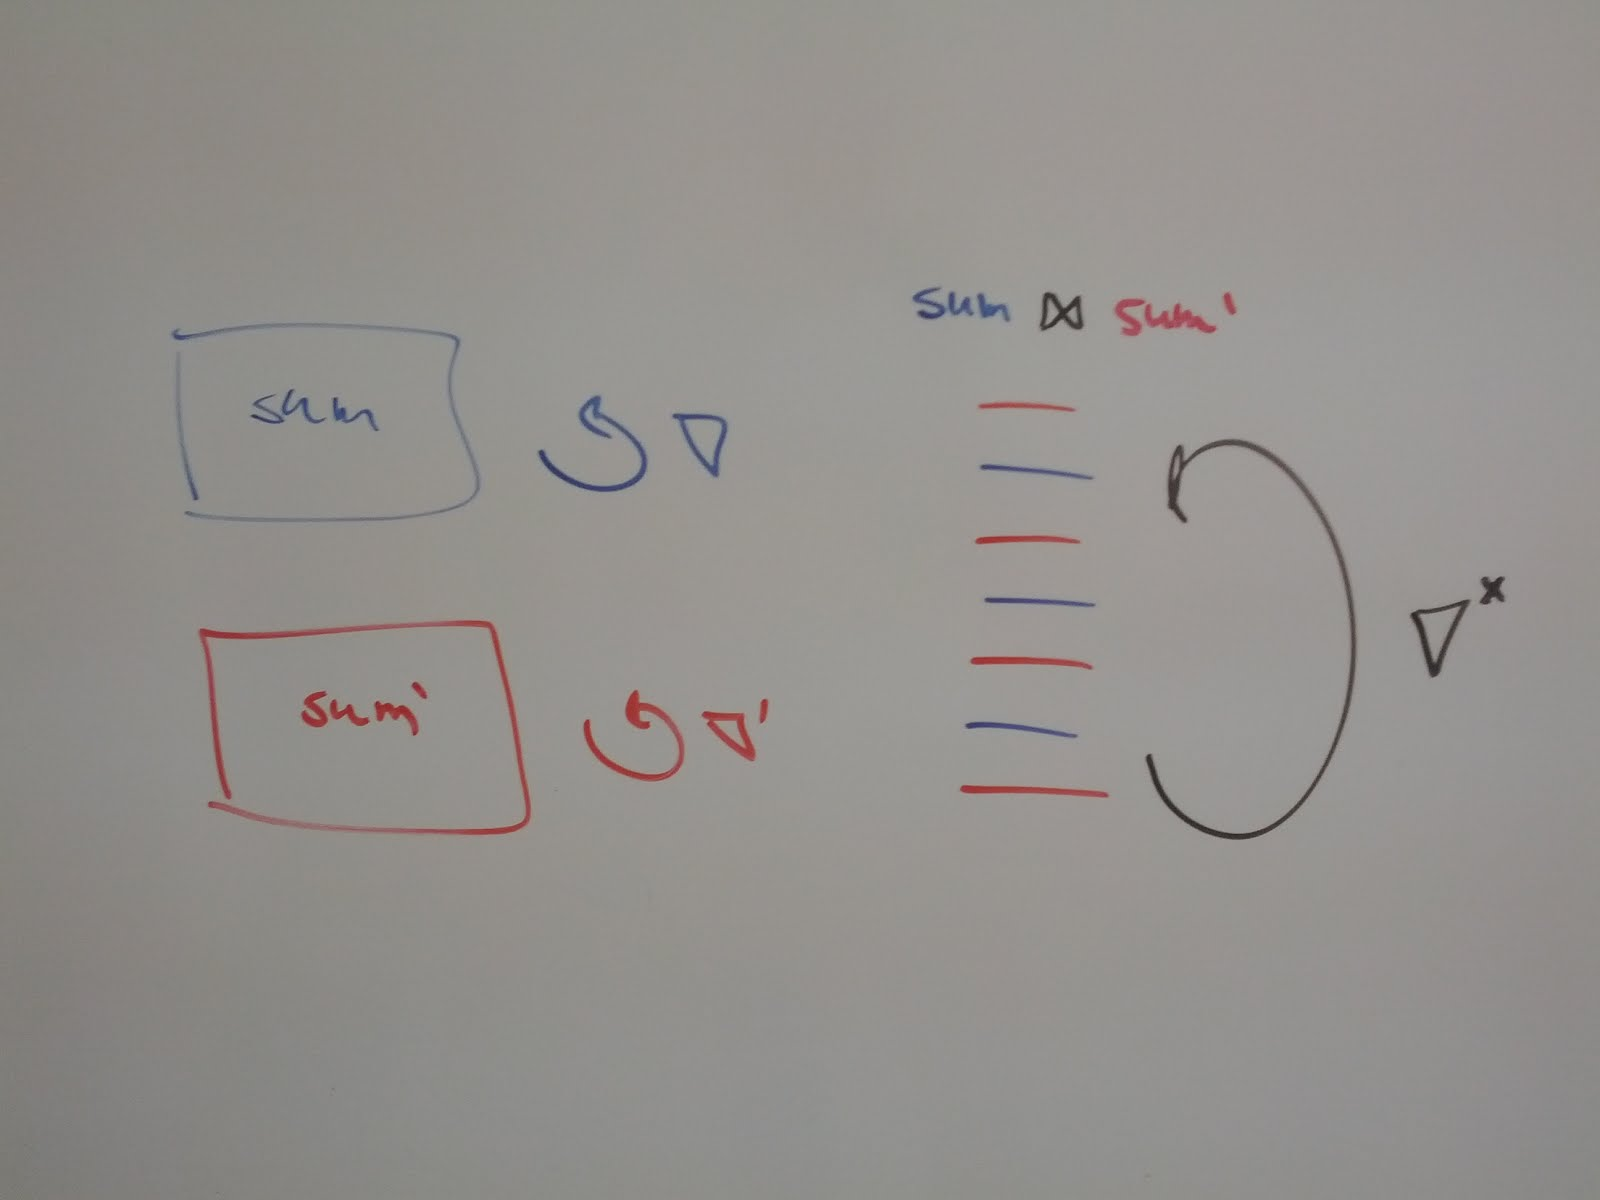
\includegraphics[scale=0.20,clip=true,trim = 150pt 250pt 200pt 200pt]{figures/sum-widening.jpg}
%}
%\caption{Widening $sum ; sum$ vs. $sum \bowtie sum$}\figlabel{SumWidening}
%\end{figure}

\paragraph{Definition of difference}
So far, we defined difference in programs as difference in output variable values at the program final state. Our work extends the notion of difference beyond that, allowing for several program locations to be identified as viable for differentiation (we name these locations \emph{differencing points} denoted $DP$). Other than the programs endpoints, we include every location which:
\begin{itemize}
\item Emits an output value (using a system function or through a global variable)
\item Accesses array
\end{itemize}
This means that procedures may now differ, even if they hold equivalence on the final state. Thus we define difference also as producing a different output value in mid-execution or accessing an array through a different index. This means that programs which differ in array access \emph{patterns} will now be flagged as different. This is a sound approach for difference, as this may include access to illegal bounds (an example for this can be seen in \figref{Md5sumExample}). We note that this definition of description cannot be achieved by instrumenting output or array access through temporary variables and deferring checking their equivalence to the end, as the amount of temporaries needed may be unbound. We therefore require procedures to agree on these locations, in case we wish to verify using the extended definition of difference.
\section{Preliminaries} \seclabel{Preliminaries}
We use the following standard concrete semantics definitions for a program:

\paragraph{Program Location / Label} \deflabel{ProgramLabel}
A program location $loc \in Loc$, also referred to as label denoted $lab$, is a unique identifier for a certain location in a program corresponding to the value of the program counter at a certain point in the execution of the program. We also define two special labels for the start and exit locations of the program as $begin$ and $fin$ respectively.

\paragraph{Concrete State} \deflabel{ConcreteState}
Given a set of variables $Var$, a set of possible values for these variables $Val$ and the set of locations $Loc$, a \emph{concrete program state} is a tuple $\sigma \triangleq \langle loc, values \rangle \in \Sigma$ mapping the set of program variables to their concrete value at a certain program location $loc$ i.e. $values : Var \rightarrow Val$. The set of all possible states of a program $P$ is denoted $\Sigma_{P}$.

\paragraph{Program} \deflabel{Program}
We describe an imperative program $P$, as a tuple $(Val,Var,\rightarrow,\Sigma_{0})$ where $\rightarrow : \Sigma_{P} \times \Sigma_{P} $  is a transition system which given a concrete program state returns the following state in the program and $\Sigma_{0}$ is a set of initial states of the program. Our formal semantics need not deal with errors states therefore we ignore crash states of the programs, as well as inter-procedural programs since our work deals with function calls by either ignoring them when equivalence was proven or by inlining them (we exclude recursion for now).

\paragraph{Concrete Trace} \deflabel{ConcreteTrace}
A program trace $\pi \in \Sigma^*_{P}$, is a sequence of states $\langle \sigma_0,\sigma_1,... \rangle$ describing a single execution of the program. Each of the states corresponds to a certain location in the program where the trace originated from. Every program can be described by the set of all possible traces for its run $\semp{P} \subseteq \Sigma^*$. We refer to these semantics as concrete state semantics. We also define the following standard operations on traces:
\begin{itemize}
\item $label : \Sigma_{P} \rightarrow Lab$ maps a state to the program label at which it appears.
\item $last : \Sigma_{P}^* \rightarrow \Sigma_{P}$ returns the last state in a trace.
\item $pre : \semp{P} \rightarrow 2^{\Sigma_{P}^*}$ for a trace $\pi$ is the set of all prefixes of $\pi$.
\item $states : \semp{P} \rightarrow 2^{\Sigma_{P}}$ for a trace $\pi$ is the set of actual states $\pi$ is composed of.
\end{itemize}


We shortly describe a \emph{product state} $\sigma_{\times} \in \Sigma_{P \times P'}$ as a pair of states $\langle \sigma,\sigma' \rangle$, a \emph{product program} $P \times P'$ as a product of the transition systems of the underlying programs and \emph{product trace} as a sequence of produce states.


\section{Concrete Semantics}\seclabel{ConcreteSem}
In this section we will define the notion of difference between concrete semantics of two programs based on a standard concrete semantics for a program.

\subsection{Concrete State Differencing} \sublabel{ConcreteDiff}
Comparing two different programs $P$ and $P'$ under our concrete semantics means comparing \emph{traces}. A trace is composed of concrete states thus we first need a way to compare states. Since a state $\sigma$ is a mapping $Var \rightarrow Val$ we need a correspondence between variables in $P$ (i.e. $Var$) and those in $P'$ (i.e. $Var'$).

\paragraph{Variable Correspondence} \deflabel{VarCorrespondence}
 A variable correspondence $VC \in Var \hookrightarrow Var'$, is a partial mapping between 2 sets of program variables. Any variable in $Var$ may be matched with one in $Var'$ and vice versa. Naturally, the comparison between states will occur between values mapped to corresponding variables, as described by $VC$.

Our experience suggests that in most cases the set of variables stays the same over subsequent versions ($Var = Var'$) and in cases where $Var$ does change, it's by the addition of new variables or removal of an old one. Therefore we concluded that for our purposes, matching variables by name is sufficient for finding a precise difference. Thus we define our standard correlation to be: $VC_Eq \equiv \{v \mapsto v' | v \in Var \wedge name(v) = name(v')\}$ and vice versa. Take notice that in cases where a variable was removed (added) by a patch, it will still be correlated to it's patched (un-patched) version, although it does not exists, and we will report it as part of the difference - this will adhere to our definition of difference. In cases where the matching is not that straightforward, for example, when variables name change, the correspondence can be generated in \TODO{a more sophisticated way}.

\paragraph{Concrete State Delta} \deflabel{ConcreteStateDelta}
Given two concrete states $\sigma \in \Sigma_P,\sigma' \in \Sigma_{P'}$ and a variable correspondence $VC$, we define the concrete state delta $\triangle_{S}(\sigma,\sigma')$ of $\sigma$ and $\sigma'$ as the part of the state $\sigma$ where corresponding variables do not agree on values (with respect to $\sigma'$). Formally: $\triangle_{S}(\sigma,\sigma') \equiv \{ (var,val) | var \in Var \wedge VC(var)=var' \wedge \sigma(var) = val \neq \sigma'(var')\}$.

We note that the state delta is not necessarily symmetric. In fact, the direction in which it is used has meaning in the context of a program $P$ and a patched version of it $P$. We define $\triangle_{S}^{-} = \triangle_{S}(\sigma,\sigma')$ which means the part of the state that was "changed" or "removed" in $P'$ and $\triangle_{S}^{+} = \triangle_{S}(\sigma',\sigma)$ which stands for the part added in $P'$.

For instance, given two states $\sigma:\{x=1,y=2,z=3\}$ and $\sigma':\{x'=0,y'=2,w'=4\}$ and assuming our default $VC$ then $\triangle_{S}^{-} = \{x=1,z=3\}$ since x and x' match and do not agree on value, y and y' agree (thus are not in delta) and no data exists for z' in $\sigma'$. Respectively, $\triangle_{S}^{+} = \{x'=0,w'=4\}$. We believe that $\triangle_{S}$ is a precise and natural definition for difference as it indeed captures the change made in the patched version. We will later on extend the definition to describe difference between abstract states.

We defined a notion for difference between states but this is insufficient to describe difference between whole runs of programs i.e. traces. Naturally, we are only interested in traces that originate from \textbf{the same input} (for the input variables correlated by $VC$) although one can contemplate the question of delta between \emph{any} two traces of a program (or two programs) however this is not the problem addressed in this paper and every mention of trace differentiation will assume the traces agree on input. The way to differentiate traces is by differentiating their states, but which states? this is not a trivial question since traces can vary in length and order of states. We need a state correspondence for choosing the states to be differentiated within the two traces. We define it as following:

\paragraph{Trace Diff Points} \deflabel{TraceDiffPoints}
Given two traces $\pi$ and $\pi'$, we define a trace index correspondence relation named trace diff points denoted $DP_{\pi}$ as a matching of indexes specifying states in where concrete state delta should be computed. Formally: $DP_{\Pi} \equiv \{(i,i')|i \in {0..|\pi|}, i' \in {0..|\pi'|}\}$.


Now that we have a way of matching states to be compared between two traces, we define the notion of trace differentiation:

\paragraph{Trace Delta} \deflabel{ConcreteTraceDelta}
 Given traces $\pi,\pi'$ of programs $P,P'$ respectively, and a state correspondence $DP_{\Pi}$ we define the trace delta $\triangle_{T}(\pi,\pi')$ as state differentiations between all corresponding states in $\pi$ and $\pi'$. Formally, for every $(i,i') \in DP$, $\triangle_{T}$ will contain the mapping $i\mapsto\triangle_{S}(\sigma_{i},\sigma'_{i'})$, thus the result will map certain states in $\pi$ to their state delta with the corresponding state' in $\pi'$ (deemed interesting by $DP_{\Pi}$). We note that $\triangle_{T}^{+}$ and $\triangle_{T}^{-}$ have a similar meaning except that now it's in a trace context.

One possible choice for $DP_{\Pi}$ would be the endpoints of the two traces $\{(fin,fin')\}$ (assuming they are finite) meaning differentiating the final states of the executions or formally: $\triangle_{in}^{-} \equiv \triangle_{Fin}(\pi,\pi') = \{fin\mapsto\triangle_{S}(\sigma_{fin},\sigma'_{fin'})\}$ (we will also be interested in $\triangle_{Fin}^{+}$). It is clear that the delta is not sufficient for truly describing the difference between said traces as it will only compare final state values and will miss out on what happened during the execution. This can be overcome by instrumenting the semantics such that the state will contain all "temporary" values for variable along with the location the values existed (by, for instance, adding temporary variables), making all the differences visible at the end point. \TODO{As a design choice we chose not to do this (since it creates many variables, choosing $VC$ here is hard, etc)}.

Defining the diff-points over any two traces is a daunting task since two traces of two separate (although similar) programs can vastly differ. If we take a look at two versions of a program depicted in \figref{MatcingProblemExamplePrograms} and the following traces generated from the input $x=2$: $\pi = \{x=2,i=0 \}\{i=1 \}\{i=2 \}$ and $\pi' = \{ x'=2,i'=0 \}\{ i'=1 \}\{ i'=2 \}\{ i'=3 \}\{i'=4\}$ (we omit labels and only mention parts of the trace where variable values change), we see that even in this simple program, finding a correlation based on traces alone is hard. However, one can get the sense that using program location as a means of correlation can produce a meaningful result. For example, if we look at all the possible values for $i$ in label $lab$ and differentiate them from the values in the patched version (in the same location), we get the meaningful result that $i$ in the patched version can range from $x+1$ up to $2x$. The need to find a label-based match, along with the need for abstraction to allow scalability, is filled by moving past the concrete trace semantics to a concrete \emph{collecting semantics}.

\begin{figure}[ht]\figlabel{MatcingProblemExamplePrograms}
\lstset{numbers=left, language=C, basicstyle=\ttfamily\scriptsize,emph={},emphstyle=\textbf,escapechar=\%}
\begin{minipage}[b]{0.5\linewidth}
\centering
\begin{lstlisting}
void foo(unsigned x) {
    unsigned i = 0;
lab:if (i >= x) return;
    i++;
    goto lab;
}
\end{lstlisting}
\end{minipage}
\hspace{0.5cm}
\begin{minipage}[b]{0.5\linewidth}
\centering
\begin{lstlisting}
void foo(unsigned x) {
    unsigned i = 0;
lab:if (i >= 2*x) return;
    i++;
    goto lab;
}
\end{lstlisting}
\end{minipage}
\caption{$P,P'$ differentiation candidates}
\end{figure}

\subsection{Differencing at Program Labels} \sublabel{DiffAtLabels}

\paragraph{Collecting Semantics of a Program Label} \deflabel{ProgramLabelCollectingSemantics}
Given a label $l \in Lab$ in a program $P$ we define the collecting semantics of a program label $states(l) \subseteq \semp{P}$ as all the concrete states that are possible at that label (i.e. exist in some trace reaching that label). Formally:
\begin{enumerate}
\item $at \equiv Lab \rightarrow (\Pi \rightarrow 2^{\semp{P}^*})$ for a given label $l$ and trace $\pi$, is the set of prefixes of $\pi$ that end in a state labeled $l$ formally: $at(l,\pi) \equiv \{\pi*|\pi* \in pre(\pi) \wedge last(\pi*)=l \}$.
\item $states(l) \equiv \{last(at(l,\pi)) | \pi \in \Pi\}$.
\end{enumerate}

Now our problem is reduced to matching the collecting semantics of labels $states(l)$. Again we are encountered with the question of how to match these labels. We note that the trace indexing correspondence $DP_{\Pi}$ defined in \defref{TraceDiffPoints} is no longer useful here as we need to differentiate sets of states belonging to a certain program label $states(l)$. Thus we require a correspondence or \emph{labels} and therefore we define the label diff points correspondence.

\paragraph{Label Diff Points} \deflabel{LabelDiffPoints}
Given two programs $P,P'$ and their sets of program labels $Lab,Lab'$, we define a label correspondence relation named label diff points denoted $DP_{Lab}$ as a matching of labels between programs. Formally: $DP_{Lab} \equiv \{(l,l')|l \in Lab, l' \in Lab'\}$.

From this point on any mention of the diff-points correspondence $DP$ will refer to label diff-points $DP_{Lab}$.

We address the question of selecting $DP_{Lab}$ in a correct and meaningful way in \subref{DiffPoints}. We will briefly mention that in order to find a meaningful correspondence, we employ a standard syntactic diff algorithm~\cite{Diff} on the two versions of the program. Our experiments show that for the purpose of differentiating versions of program, this approach works well since patched versions tend to be syntactically similar (especially when the versions come from two successive check-ins to the code repository).

Given the correspondence of labels in $P$ and $P'$ (from $DP$), we now know which $states(l)$ and $states(l')$ we need apply delta on. Delta is now applied on \emph{sets} of states, which is defines by simply applying the state delta \defref{ConcreteStateDelta} between each of the states in both states and removing from the result matched states or formally: $\triangle_{C}(states(l) ,states(l')) \equiv \{\sigma \in states(l)| \neg \exists \sigma' \in states(l') \cdot \triangle_{S}(\sigma, \sigma') = \emptyset\}$

For example, given two sets of states $C : \{\sigma_1:\{x=0,y=0\},\sigma_2:\{x=1,y=2\}\}$ and $C' : \{\sigma'_1:\{x=0,y=0\},\sigma'_2:\{x=4,y=5\}\}$ and using $VC_Eq$ then $\triangle_{C}^{-} = \{\{x=1,y=2\}$ and $\triangle_{C}^{+} = \{\{x=4,y=5\}\}$. Note that $\triangle_{C}^{+}$ now obtains the meaning of "lost states" as in states which existed in the previous version and removed by the patch (similarly $\triangle_{C}^{-}$ here means "new states").

We must remember however, that the sets of states to be compared are potentially unbounded which means that the delta we compute may be unbounded too. Therefore we must use an abstraction over the collecting semantics that will allow us to represent the collecting semantics in a bounded way.

\section{Abstract Correlating Semantics}\seclabel{AbstractSem}

In this section, we introduce our correlating abstract domain which allows bounded representation of product program state while maintaining equivalence between correlated variables. This comes at the cost of an acceptable lose of precision of other state information. We represent variable information using standard relational abstract domain. As our analysis is path sensitive, we allow for a set of abstract sub-states, each adhering to a certain path in the product program. This abstraction is similar to the trace partitioning domain as described in \cite{MauborgneRival07}. To assure we only consider correlated paths from the product programs (that agree on input), our abstraction will initially assume equality on all inputs. This power-set domain records precise state information but does not scale due to exponential blow-up of number of paths. To reduce state size, we define a special join operation that dynamically partitions the abstract state according to the set of equivalences maintained in each sub-state and joins all sub-states in the same partition together (using the sub-domain lossy join operation). This equivalence criteria allows separation of equivalence preserving paths thus achieving better precision. We start off by abstracting the correlating trace semantics in \ssecref{ConcreteCorrelatingSemantics}.

In the following, we assume an abstract relational domain $(\A{D}, \sqsubseteq_{D})$ equipped with operations $\sqcap_{D}$, $\sqcup_{D}$ and $\nabla_{D}$, for representing sets of concrete states in $\Sigma_{P \times P'}$. We separate the set of program variables into original program variables denoted $Var$ (which also include a special added variable for return value, if such exists) and the added guard variables denoted $Guard$ that are used for storing conditional values alone ($Guard$ also include a special added variable for return flag). We assume the abstract values in $\A{D}$ are constraints over the variables and guards (we denote $\A{D}_{Guard}$ for abstraction of guards and $\A{D}_{Var}$ for abstracting original variables), and do not go into further details about the particular abstract domain as it is a parameter of the analysis. We also assume that the sub-domain $\A{D}$ allows for a sound over-approximation of the concrete semantics (given a sound interpretation of program operations). In our experiments, we use the polyhedra abstract domain~\cite{CousotHalbwachs78} and the octagon abstract domain~\cite{Mine07}.

\paragraph{Correlating Abstract State} \deflabel{CorrelatingAbstractState}
A correlating abstract program state $\A{\sigma} \in Lab_{\times} \rightarrow 2^{\A{D}_{Guard} \times \A{D}_{Var}}$, is a set of pairs $\langle ctx, data \rangle \in \C{\Sigma}$ mapped to a product program label $l_{\times}$, where $ctx \in \A{D}_{Guard}$ is the execution context i.e. an abstraction of guards values via the relational numerical domain and $data \in \A{D}_{Var}$ is an abstraction of the variables (anything that is not a guard) also using the domain $\A{D}$. We separate abstractions over guard variables added by the transformation to GCL and original program variables as there need not be any relationships between guard and regular variables.

\begin{table}
\footnotesize
\renewcommand{\arraystretch}{1.4}
\begin{tabular}{lcl}
\hline
$\asemp{v:=e}$ & \hspace{0.1in} & $l_{\correlate} \mapsto \{\langle ctx,\asemp{v:=e}_{\A{D}}(data) \rangle | \langle ctx,data \rangle \in S \}$
\\
\hline
$\asemp{g:=e}$ & & $l_{\correlate} \mapsto \{\langle \asemp{g:=true}_{\A{D}}(ctx),\asemp{e}_{\A{D}}(data) \rangle  | \langle ctx,data \rangle) \in S \}$ \\
& & ~~~~~~~~~~~$\cup \{ \langle \asemp{g:=false}_{\A{D}}(ctx),\asemp{\neg e}_{\A{D}}(data) \rangle | \langle ctx, data \rangle \in S \}$
\\ \hline
$\lsyn$ \textbf{if} (g) $\{s_{0}\}$ \textbf{else} $\{s_{1}\}$ $\rsyn^{\sharp}$ & &
$l_{\correlate} \mapsto \{\langle\asemp{g=true}_{\A{D}}(ctx),  \asemp{s_0}_{\A{D}}(data) \rangle | \langle ctx,data \rangle) \in S \}$ \\
& & ~~~~~~~~~~~$\cup \{\langle \asemp{g=false}_{\A{D}}(ctx), \asemp{s_1}_{\A{D}}(data) \rangle | \langle ctx,data \rangle \in S \}$
\\ \hline
$\lsyn$ \textbf{goto} lab $\rsyn^{\sharp}$ & & $\A{\sigma}$
\\ \hline
\end{tabular}
\renewcommand{\arraystretch}{1}
\caption{Abstract transformers}\label{Ta:AbsTrans}
\end{table}


\paragraph{Correlating Abstract Semantics} \deflabel{CorrelatingAbstractSemantics}
\tabref{AbsTrans} describe the abstract transformers. The table shows the effect of each statement on a given abstract state $\A{\sigma} = l_{\times} \mapsto S$. The abstract transformers are defined using the abstract transformers of the underlying abstract domain $\A{D}$.

We assume that any program P can be transformed such that it contains only the aforementioned operations (specifically GCL format). We also assume that for $\asemp{g:=e}$ operations, $e$ is a logical operation with binary value.
Next, we define the abstraction function $\alpha : 2^{\Sigma^{*}_{times}} \rightarrow 2^{\A{D} \times \A{D}}$ for a set of concrete traces $T \subseteq \Sigma^{*}_{times}$. As in our domain traces are abstracted together if they share the exact same path, we first define an operation $path : \Sigma^{*}_{times} \rightarrow Lab^{*}$ which returns a sequence of labels for a trace's states i.e. what is the path taken by that trace. We also allow applying $path$ on a set of traces to denote the set of paths resulting by applying the function of each of the traces. Finally: $\alpha(T) \triangleq \{ \sqcup_{path(\pi)=p} \beta(last(\pi)) | p \in path(T) \}$ where $\beta(\C{\sigma}) = \langle \beta_{\A{D}}(\C{\sigma}|_Guard), \beta_{\A{D}}(\C{\sigma}|_{Var}) \rangle$  i.e. applying the the abstraction function of the abstract sub-domain $\beta_{\A{D}}$ on parts of the concrete state applying to $Guards$ and $Vars$ separately. Our abstraction partitions trace prefixes $\pi$ by path and abstracts together the concrete states reached by the prefix - $last(\pi)$, using the sub-domain.

%such that each $rd \in S_{RD}$ will abstract a certain \textbf{path} in the product program. We achieve that by instrumenting each $\sigma_{\times} = last(pre(\pi_{\times}))$ in the collecting semantics $CS(l_{\times})$ with the sequence of branches taken up to $\sigma_{\times}$ in $pre(\pi_{\times})$. This is easily achieved by using \emph{guard} values as they are recorded along the trace and we denote $path(\sigma_{\times})$ as the sequence of branches $b_0,...,b_n$ i.e. guard values ($b_i = <g,{T/F}>$), that led up to $\sigma_{\times}$. Therefore we define for every path $p_i$ in the product program the group of concrete correlating states that exist at the end of that path denoted $\Sigma_{\times}^{p_i} \triangleq \{ \sigma_{\times} | path(\sigma_{\times}) = p_i \}$. Finally we define the abstract state itself as $\C{\sigma_{\times}} \triangleq { rd | rd = ABS_{RD}(\Sigma_{\times}^{p_i}) \wedge p_i is a path in P \times P)}$. For example, the abstraction of \figref{MatchingProblemExamplePrograms}'s product program collecting semantics at labels $(lab,lab')$ will first collect together all trace prefixes that iterate the loop 0 times: $\Sigma_{\times}^{p_0} = \{  (x=0,i=0,x'=0,i'=0), (x=1,i=0,x'=1,i'=0), (x=2,i=0,x'=2,i'=0), ... \}$ and abstract them using the relational sub-domain to get $rd_{0} = \{x=x',i=i'=0\}$ which correctly expresses the fact that equivalence is kept in case none of the loops iterate. The next path to be abstracted would be where both loops iterate once i.e. $p_1 = <g,F>,<g',F>$ which also maintains equivalence and will be abstracted as $rd_{1} = \{x=x',i=i'=1, x \geq 1\}$. The next path however, which iterates the $P'$ loop twice but only once for the $P$ loop, $p_2 = <g,F>,<g',F>,<g,T>,<g',F>$ will not maintain equivalence as it will abstract $\Sigma_{\times}^{p_2} = \{  (x=1,i=1,x'=1,i'=2), (x=2,i=2,x'=2,i'=2), (x=3,i=2,x'=3,i'=2), ... \}$ as $rd_{2} = \{x=x',2 \leq i \geq 1, i'=2\}$. We mention that the abstract $rd$ ignores the separation of concrete states of $P$ and $P'$ and abstracts both variable data together. In fact, the ability to maintain direct relationships between the two sets of variables (and specifically those matched by $VC$) is crucial for maintaining equivalence.

Every path in the product program will be represented by a single sub-state of the sub-domain. As a result, all \emph{traces prefixes} that follow the same path to $l_{\times}$ will be abstracted into a single sub-state of the underlying domain. This abstraction fits semantics differencing well, as inputs that follow the same path display the same behavior and will usually either keep or break equivalence together, allowing us to separate them from other behaviors (it is possible for a path to display both behaviors as in \figref{PathProblemExamplePrograms} and we will discuss how we are able to manipulate the abstract state and separate equivalent behaviors from ones that offend equivalence). Another issue to be addressed is the fact that our state is still potentially unbound as there may be an infinite number of paths in the program (due to loops).

%\paragraph{Computing Abstract State with Our Analysis} \deflabel{ComputingAbstractState}
%We compute the correlating abstract state at each label $\C{\sigma_{\times}}$ by using means of abstract interpretation and program analysis. We interpret our correlating program (described in \secref{CorrelatingProgram}) which is a semantic preserving reduction over the much more arbitrary product program, using a standard fixed-point analysis algorithm, and apply interpreted operations on the set of sub-states of the current state $S_{RD}$. Our initial state explicitly assumes equality on all input variables (by adding a $v=v'$ constraint for every input variable $v$ where $v'=VC(v)$) to allow for sound checking of equivalence. This also allows for pruning of unfeasible paths where inputs diverge\COMMENT{ (though we may still interpret some as feasible due to incompleteness of program operations representation, for example bitwise operations)}. To adhere to the representation of traces in the abstract state, our join operation is in fact set union, thus indeed every prefix that reaches a certain program label will be awarded its own $rd$. Let us explicitly define the operations of the domain in our analysis:
%\begin{itemize}
%\item $S^{RD}_1 \sqsubseteq S^{RD}_2 \Longleftrightarrow \forall rd_1 \in G_1 \exists rd_2 \in G_2 : rd_1 \sqsubseteq_{RD} rd_2$
%\item $S^{RD}_1 \sqcap S^{RD}_2 \equiv { rd_1 \sqcap_{RD} rc_2 | rd_1 \in G_1 \wedge rd_2 \in G_2}$
%\item $S^{RD}_1 \sqcup S^{RD}_2 \equiv S^{RD}_1 \cup S^{RD}_2$
%\end{itemize}
%Next we define two more operations: Canonization (denoted $\odot$) - which allows for minimization of state size according to equivalence criteria and Widening (denoted $\nabla$) - which allows reaching a fixed-point when handling loops.

%\COMMENT{One advantage of our correlating domain over using two separate domains, is the ability to preserve equivalence in the face of non-linear operations - this argument may be too thin to include.}

\begin{figure}
\centering
\begin{tabular}{cc}
\begin{lstlisting}
int f(int x) {
    return x;
}
\end{lstlisting}
\hspace{1cm}
&
\begin{lstlisting}
int f'(int x) {
    return 2*x;
}
\end{lstlisting}
\end{tabular}
\caption{Single path differentiation candidates}
\figlabel{PathProblemExamplePrograms}
\end{figure}


\paragraph{Partitioning}
Performing analysis with the powerset domain does not scale as the number of paths in the correlated program may be exponential. We must allow for reduction of state $\A{\sigma} = l_{\times} \mapsto S$ with acceptable loss of precision. This reduction via partitioning can be achieved by joining the abstract sub-states in $S$ (using the standard precision losing join of the sub-domain) but to perform this we must first answer the following: (i) which of the sub-states shall be joined together and (ii) at which program locations should the partitioning occur. A trivial partitioning strategy is simply reverting back to the sub-domain by applying the join on all sub-states which may result in unacceptable precision loss as exemplified in \figref{SignCorrelating}. However, by taking a closer look at the final state of the same example:
\\
\begin{tabular}{c}
$\A{\sigma}(fin)$ = [
\\
$\langle (g1=1,g2'=0,\equiv_{g1}),(sgn=1,\equiv_{x,sgn}) \rangle$,
\\
$\langle (g1=0,g2'=0,\equiv_{g1}), (x<0,sgn=-1,\equiv_{x,sgn}) \rangle$,
\\
$\langle (g1=0,g2'=1,\equiv_{g1}),(x=0,sgn=0,sgn'=1,\equiv_{x}) \rangle$
\\
]
\end{tabular}
\\
One may observe that were we to join the two sub-states that maintain equivalence on $\{x,sgn,g1\}$, it would result in an acceptable loss of precision (of losing the $x$ related constraints). This is achieved by partitioning sub-states according to the set of variables which they preserve equivalence for. This bounds the state size at $2^{|V|}$, where $V$ is the set of correlating variables we wish to track.
As mentioned, another key factor in preserving equivalence and maintaining precision is the program location at which the partitioning occurs. The first possibility, which is somewhat symmetric to the first proposed partitioning strategy, is to partition at every join point i.e. after every branch converges. A quick look at \figref{SignCorrelating}'s state after processing the first guarded instruction \scode{if (G1) sgn = -1;}, i.e (we ignored $g2'$ effect at this point for brevity):
\\
\begin{tabular}{c}
$\A{\sigma}$ = [
\\
$\langle (g1=0,\equiv_{g1}),(x \geq 0,\equiv_{x,sgn}) \rangle$,
\\
$\langle (g1=1,\equiv_{g1}),(x < 0,sgn' = -1, \equiv_{x}) \rangle$
\\
\end{tabular}
\\
suggests that partitioning at join points will perform badly in many scenarios, specifically here as we will lose all data regarding $sgn$. However if we could delay the partitioning to a point where the two programs "converge" (after the following \scode{if (G1') sgn' = -1;} line), we will get a more precise temporary result which preserves equivalence. Therefore we define another partitioning points, which are defined during the correlating program construction process described in \secref{Correlating}, and are basically locations where the two (guarded) programs have syntactically converged (we found two lines that are syntactically equal, sans tagging). Another possible location for differencing are our \emph{differencing points}. Partitioning at these locations is essentially more precise than at correlation points. We remind that diff-points are product program locations where both programs conceptually converge as they are about to emit output i.e. both programs have finished "preparing" the next portion of output therefore, if equivalence exists - it must exist now, therefore this is a prime candidate for a partitioning point. \TODO{Our evaluation includes applying each of our strategies along with each of the points. Intuitively, the results should range from least precise using the <Join-All,At-Join> strategy and point to most precise in the <Join-Equiv,At-Diff> scenario and this is indeed the case as we show in \secref{Evaluation} (not taking into account the no-partitioning scenario which is naturally most precise).}


%We can see from our motivating example that it is not feasible to allow our correlating domain to keep diverging and double in size with every conditional as it will exponentially blow up the analysis run-time and memory. Instead, we employ an equivalence conserving canonization technique such that at every canonization point we will partition the sub-states according to the set of variables to which they hold equivalence for and join these all together into one abstract, using the sub-domain lossy join. This bounds the number of abstracts in the state to $2^{|V|}$ for variables correlated $VC$. This fine grained equivalence checking is successful in telling apart paths that hold equality for none, some or all of the variables. For instance in \figref{MatchingProblemExamplePrograms}, our canonization will tell apart the sub-state that hold equivalence for all variables $\{i=i'=x=x'=0\}$ from the rest that hold equivalence for $x$ alone and join them all together into the $\{x=x',i \leq x, i' \leq 2x'\}$ state. The fact that we did not lose equivalence altogether is beneficial as we are able to report that the input variable $x$ did not diverge which may be of use in case \scode{foo} had used $x$ further down the road.

\begin{figure}
\centering
\begin{tabular}{c}
\begin{lstlisting}
unsigned max = ...;
int sum''(int arr[], unsigned len) {
  int result = 0;
  if (len > max)
    return -1;
  for (unsigned i = 1; i < len; i+=2)
    result += arr[i];
 return result;
}
\end{lstlisting}
\\
\\ \hline
\\
\begin{lstlisting}
unsigned max' = ...;
int sum(int arr[], unsigned len) {
  unsigned len' = len;
  int arr'[] = arr;
  int result = 0;
  int result' = 0;
  guard r' = (len' > max');
  if (r') retval' = -1;
  if (r') r' = 0;
  {
    unsigned i = 1;
    unsigned i' = 1;
l:  guard g = (i < len);
l': guard g' = (i' < len');
    if (g) result += arr[i];
    if (r') if (g') result' += arr'[i'];
    if (g) i+=2;
    if (r') if (g') i'+=2;
    if (g) goto l;
    if (r') if (g') goto l';
  }
}
\end{lstlisting}
\end{tabular}
\caption{Patched $sum'$ and correlating $sum \bowtie sum''$}
\figlabel{LoopCorrelatingExample2}
\end{figure} 

\paragraph{Widening}
In order for our analysis to handle loops we require a means for reaching a fixed point. As our analysis advances over a loop and state is transformed, it may keep changing and never converge unless we apply the widening operator to further over-approximate the looping state and arrive at a fixed point. We have the widening operator of our sub-domain at our disposable, but again we are faced with the question of how we apply this operator, i.e. which pairs of sub-states $\langle ctx , data \rangle$ from $\A{\sigma}$ should be widened with which. A first viable strategy, similar to the first partitioning strategy, is to perform an overall join operation on all pairs which will result in a single pair of sub-states and then simply apply the widening to this sub-state using the sub-domain's $\nabla$ operator. If we examine applying this strategy to $sum \bowtie sum$ from \figref{LoopCorrelatingExample}, we see that it will successfully arrive at a fixed point that also maintains equivalence as all sub-states maintain equivalence at loop back-edges. Now let us try applying the strategy to the more complex $sum \bowtie sum'$ as seen in \figref{LoopCorrelatingExample}. First we mention that as $sum'$ introduces a return statement under the $len > max$ condition, the example shows an extra $r'$ guard for representing a return (this exists in all GCL programs but we omitted it so far for brevity). While analyzing, once we pass that first conditional, our state is split to reflect the return effect:
\\
\begin{tabular}{c}
$\A{\sigma}$ = [
\\
$c_1 = \langle$ (r' = 1),(len = len' > max, return\_value' = -1, result = result' = 0) $\rangle$
\\
$c_2 = \langle$ (r' = 0),(len = len' < max, result = result' = 0) $\rangle$
\\
]
\end{tabular}
\\
As we further advance into the loop, $c_2$ will maintain equivalence but $c_1$ will continue to update the part of the state regarding un-tagged variables  (since $r'=1$ in $c_1$ and it will not consider any of the commands guarded by $r'$), specifically it will change $result$ continuously, preventing the analysis from reaching fixed point. We would require widening here but using the naive strategy of a complete join will result in aggressive loss of precision, specifically losing all information regarding $result$. The problem originates from the fact that prior to widening, we joined sub-states which adhere to two different loop behaviors: one where both $sum$ and $sum'$ loop together (that originated form $len < max$) and the other where $sum'$ has existed but $sum$ continues to loop ($len \geq max$). Ideally, we would like to match these two behaviors and widen them accordingly. We devised a widening strategy that allows to do this as it basically matches sub-states that adhere to the same behavior, or loop-paths. We do this by using \emph{guards} for the matching. If two sub-states agree on their set of guards, it means they represent the same loop path and can be widened as the latter originated from the former (widening operates on subsequent iterations). In our example, using this strategy will allow the correct matching of states after consequent $k, k+1$ loop iterations:
\\
\begin{tabular}{c}
$\A{\sigma}_{k}$ = [
\\
$c_1 = \langle$ (r' = 1,g=1,g'=0),
\\
(len = len' > max, return\_value' = -1,
 result' = 0,result = $\Sigma_{i=0}^{k} arr[i]) \rangle$
\\
$c_2 = \langle$ (r' = 0,g=1,g'=1),
\\
(len = len' < max, result = result' = $\Sigma_{i=0}^{k} arr[i]) \rangle$
\\
]
\end{tabular}
\\
And:
\\
\begin{tabular}{c}
$\A{\sigma}_{k+1}$ = [
\\
$c_1 = \langle$ (r' = 1,g=1,g'=0),
\\
(len = len' > max, return\_value' = -1,
 result' = 0,result = $\Sigma_{i=0}^{k+1} arr[i]) \rangle$
\\
$c_2 = \langle$ (r' = 0,g=1,g'=1),
\\
(len = len' < max, result = result' = $\Sigma_{i=0}^{k+1} arr[i]) \rangle$
\\
]
\end{tabular}
\\
As we can identify the states predecessors by simply matching the guards. $c_1$ will be widened for a precise description of the difference shown as $\langle len = len' > max, return\_value' = -1, return\_value' = \top \rangle$.

\subsection{Correlating Abstract State Differencing} \sseclabel{CorrelatingAbstractDiff}
Given a state in our correlating domain, we want to determine whether equivalence is kept and if so under which conditions it is kept (for partial equivalence) or determine there is difference and characterize it. As our state may hold several pairs of sub-states, each holding different equivalence data, we can provide a verbose answer regarding whether equivalence holds. We partition our sub-states according to the set of variables they hold equivalence for and report the state for each equivalence partition class. Since we instrument our correlating program to preserve initial input values, for some of these states we will also be able to report input constraints thus informing the user of the input ranges that maintain equivalence. In the cases where equivalence could not be proved, we report the offending states and apply a differencing algorithm for extraction of the delta. \figref{PathProblemExamplePrograms} shows an example of where our analysis is unable to prove equivalence (as it is sound), although part of the state does maintain equivalence (specifically for $x=0$). This is due to the abstraction being to coarse. We describe an algorithm that given a sub-state $d \in \A{D}$, computes the differentiating part of the sub-state (where correlated variables disagree on values) by splitting it into parts according to equivalence. This is done by treating the relational constraints in our domain as geometrical objects and formulating delta based on that.

\paragraph{Correlating Abstract State Delta} \deflabel{CorrelatingAbstractStateDelta}
Given a sub-state $d$ and a correspondence $VC$, the correlating state delta $\triangle_{A}(d)$, computes abstract state differentiation over $d$. The result is an abstract state $\sqsubseteq rd$ approximating all concrete values for variables correlated by $VC$, that differ between $P$ and $P'$. Formally, the delta is simply the abstraction of the concrete trace deltas $\alpha(\cup_{path}\triangle_{T}^{+}), \alpha(\cup_{path}\triangle_{T}^{-})$ where deltas are grouped together by path and then abstracted. But it is not clear as to how we compute this set differencing on the correlating abstraction. Instead, we consider the geometric representation of the domain and applied operations there for the extraction of delta, as following:
\begin{enumerate}
\item $d_{\equiv}$ is a state abstracting the concrete states shared by the original and patched program. It is achieved by computing: $d_{\equiv} \triangleq d|_{V=V'} \equiv d \sqcap \bigwedge\{ v = v' | VC(v) = v'\}$.
\item $\overline{d_{\equiv}}$ is the negated state i.e. $\A{D} \setminus d_{\equiv}$ and it is computed by negating $d_{\equiv}$ (as mentioned before, all logical operations, including negation, are defined on our representation of an abstract state).
\item Eventually: $\triangle_{A}(d) \triangleq d \sqcap \overline{d_{\equiv}}$ abstracts all states in $P \times P'$ that where correlated variables values do not match.
\item $\triangle_{A}(d)^{+} = \triangle_{A}(d)|_{V'}$ is a projection of the differentiation to display values of $P'$ alone i.e. "added values".
\item $\triangle_{A}(d)^{-} = \triangle_{A}(d)|_{V}$ is a projection of the differentiation to display values of $P$ alone i.e. "removed values".
\end{enumerate}
Applying the algorithm on \figref{PathProblemExamplePrograms}'s $P$ and $P'$ where $rd = \{ retVal' = 2retVal \}$ will result in the following:
\begin{enumerate}
\item $d_{\equiv} = \{ retVal' = 0, retVal = 0 \}$.
\item $\overline{d_{\equiv}} = [ \{ retVal' > 0 \}, \{ retVal' < 0 \}, \{ retVal > 0 \}, \{ retVal < 0 \} ]$
\item $\triangle_{A}(d)  = [ \{ retVal' = 2retval, retVal' > 0 \}, \{ retVal' = 2retval, retVal' < 0 \}, \{ retVal' = 2retval, retVal > 0 \}, \{ retVal' = 2retval, retVal < 0 \} ]$
\item $\triangle_{A}(d)^{+} = [ \{ retVal' > 0 \}, \{ retVal' < 0 \} ]$
\item $\triangle_{A}(d)^{-} = [\{ retVal > 0 \}, \{ retVal < 0 \}]$
\end{enumerate}
We see that displaying the result in the form of projections is ill-advised as in some states differentiation data is represented by relationships on correlated variables alone, thus projecting will lose all data and we will be left with a less informative result. A geometrical representation of $\triangle_{A}$ calculation can be seen in \figref{Delta}.

\begin{figure}
\imagetop{
%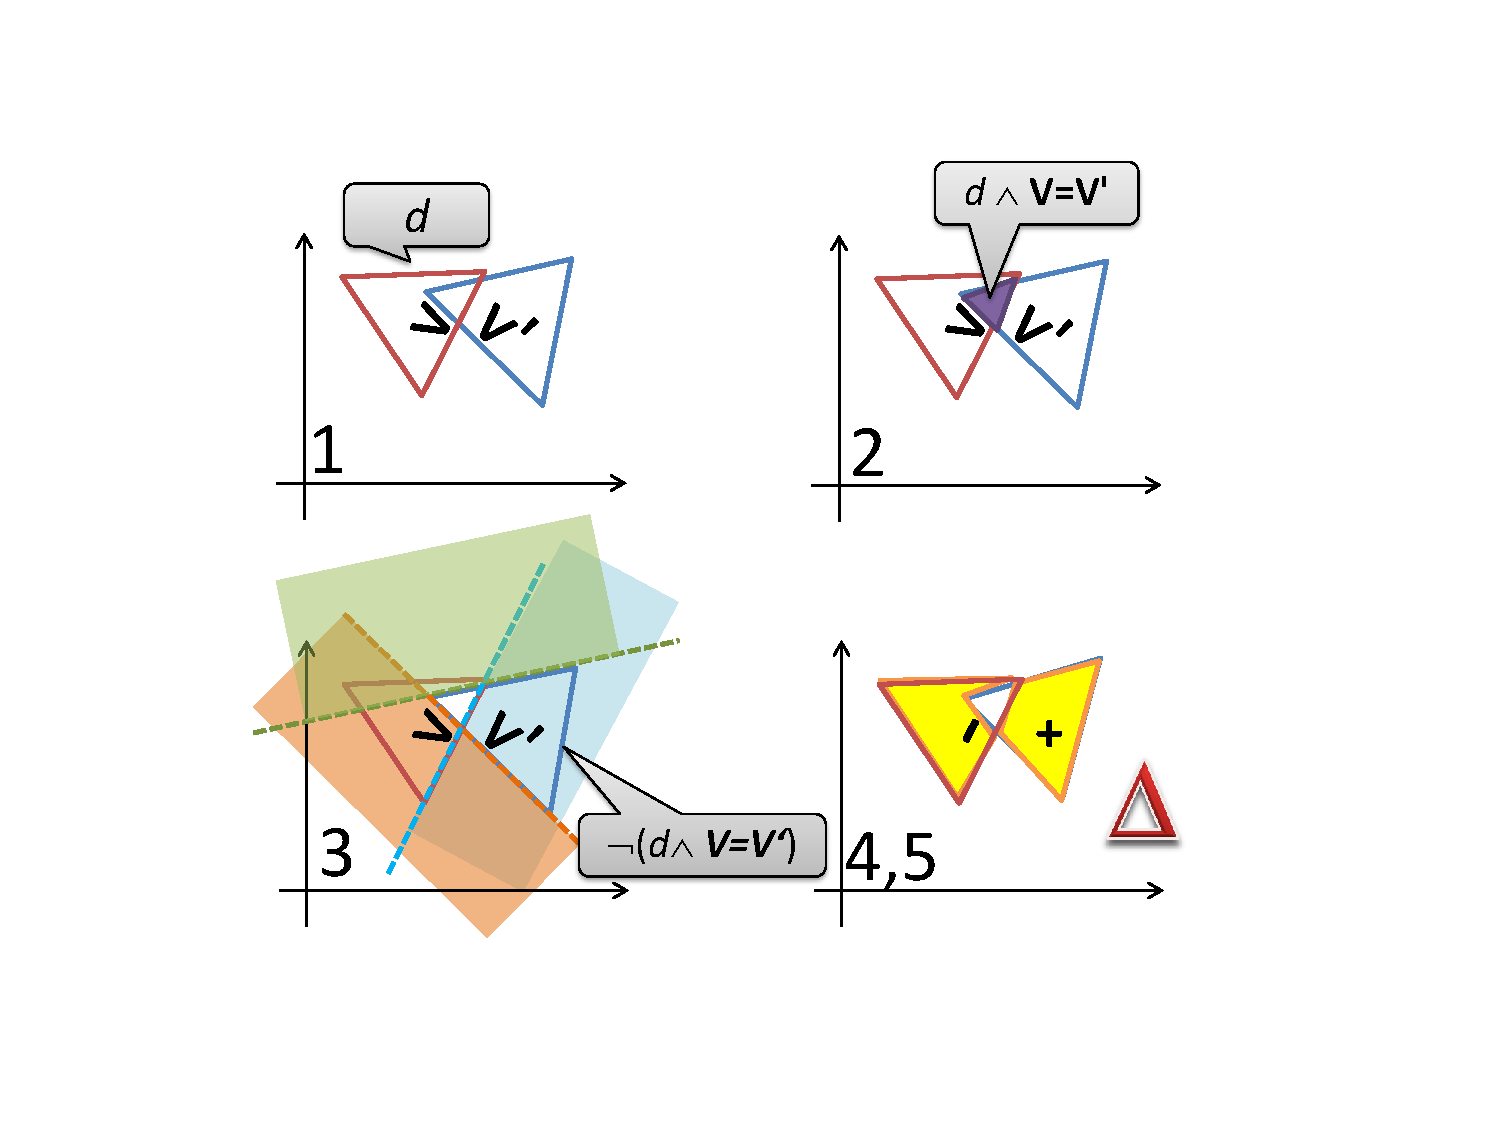
\includegraphics[width=3.0in,clip=true,trim = 100pt 100pt 300pt 300pt]{figures/delta}
}
\caption{Delta computation geometrical representation.}\figlabel{Delta}
\end{figure}

%\begin{algorithm}
\small
\DontPrintSemicolon
%\linesnumbered
\SetAlgoLined
\SetAlgoSkip{bigskip}
\KwIn{Abstract state $rd$}
\KwOut{Abstract difference - $\triangle(rd)$}
$rd_{\equiv} \leftarrow rd \sqcap \bigwedge\{ v = v' | VC(v) = v'\}$\;
$\overline{rd_{\equiv}} \leftarrow \neg rd_{\equiv} = \{ \neg c | c \in rd_{\equiv}\}$\;
Foreach $rd_i \in \overline{rd_{\equiv}}$:
    $\triangle(rd) \leftarrow \triangle(rd) \cup (rd \sqcap rd_i$)\;
\Return $\triangle(rd)$
\caption{Compute Abstract Difference.}\label{Alg:AbsDiff}
\end{algorithm}
%% RESET THE ALGORITHMS COUNTER TO PUSHBACK INC FROM FUNCTIONS
\setcounter{algocf}{1}


From this point forward any mention of 'delta' (denoted $\triangle$) will refer to the correlating abstract state delta (denoted $\triangle_{A})$. We claim that $\triangle$ is a correct abstraction for the concrete state delta which allows for a scalable representation of difference we aim to capture.

\section{Correlating Program} \seclabel{Correlating}

In this section we describe how we construct a correlating program $P \bowtie P'$. The process of correlating attempts to find a interleaving of programs for a more precise differentiation. The building process also instruments $P \bowtie P'$ with the required correlation points $CP$ which define the locations for our partitioning. We also allow a user defined selection of $CP$.

\subsection{Construction of $P \bowtie P'$ }\sseclabel{CorrelatingProgramConstruction}
The idea of a correlating program is similar to that of
self-composition~\cite{AikenTerauchi05}, but the way in
which statements in the correlating program are combined is designed to
keep the steps of the two programs close to each other. Analysis of the correlating program can then recover equivalence between values of correlated variables even when
equivalence is \emph{temporarily} violated by an update in one version, as
the corresponding update in the other version follows shortly thereafter.

We will generally describe the process of constructing the correlating program. The correlating program is an optimized reduction over $P \times P'$ where not all pairs of $(\A{\sigma},\A{\sigma'})$ are considered, but only pairs that result from a controlled execution, where correlating instructions in $P$ and $P'$ will execute adjacently. This will allow for superior precision.

The input for the correlation process are two program $(P,P')$ in C\footnote{The C programming language}. The first step involves transforming both programs to a normalized guarded instruction form $(P_{G},P'_{G})$. Next, a vector of \emph{imperative commands} $I$ (and $I'$ respectively) is extracted from each program for the purposes of performing the syntactic diff. An imperative command in our GCL format is defined to be either one of \scode{v := e | goto l | f(...)} as they effectively change the program state (variable values, excluding guards) and control. Function calls are either inlined, in case equivalence could not be proven for them, or left as is, in case they are equivalent or are external system calls. Continuing the construction process, a syntactical diff~\cite{HuntMcIlroy75} is computed over the vectors $(I,I')$. One of the inputs to the diff process is $VC$ as it is needed to identify correlated variables and the diff comparison will regard commands differing by variable names which are correlated by $VC$ as equal. The result of the last step will be a vector $I_{\diff}$ specifying for each command in $I,I'$ whether it's an added command in $P'$ (for $I'$) marked $+$, a deleted command from $P$ (for $I$) marked $-$, or a command existing in both versions marked $=$. This diff determines the order in which the commands will be interleaved in the resulting $P \bowtie P'$ as we will iterate over the result vector $I_{\diff}$ and use it to construct the correlating program. We remind that since $I,I'$ contain only the imperative commands, we cannot use it directly as $P \bowtie P'$. Instead we will use the imperative commands as markers, specifying which chunk of program from $P_G$ or $P'_G$ should be taken next and put in the result. The construction goes as follows: iterate over $I_{\diff}$ and for every command $c$ ($c'$) labeled $l_c$ ($l_{c'}$):
\begin{itemize}
\item read $P_G$ ($P'_G$) up to label $l_c$ ($l_{c'}$) including into block $B_c$ ($B_c'$)
\item for $B_c'$, tag all variables in the block.
\item emit the block to the output.
\item delete $B_c$ ($B_c'$) from $P_G$ ($P'_G$).
\end{itemize}
The construction is now complete. We only add that at the start of the process, we strip $P'_G$ of its prototype and add declarations for the tagged input variables, initializing them to the untagged version (thus assuring $P \correlate P'$ will only co-execute traces that originate from the same input for $P$ and $P'$).
As mentioned $CP$ is also a product of the construction, and it's defined using $=$ commands: after two $=$ commands are emitted to the output, we add an instrumentation line, telling the analysis of the correlation point.
One final observation regarding the correlating program is that it is a legitimate program that can be run to achieve the effect of running both versions. We plan to leverage this ability to use dynamic analysis and testing techniques such as fuzzing~\cite{NethercoteSeward07} and directed automated testing~\cite{CadarDunbarEngler08} on the correlating program in our future work.

%%\section{Abstract Interpretation of Union Programs} \label{Se:Interpretation}
In this section we explore the use of abstract interpretation techniques for differential analysis. We will first suggest an imprecise naive analysis using a simple convex domain. Then we will show how a more complicated domain allows for a precise result but is computationally infeasible. Finally we will describe our method for fine-tuning the domain to receive a scalable interpretation that manages to preserve equivalence thus being precise.

\subsection{Naive Differential Analysis}\label{Se:Naive}
Our first attempt at analyzing a union program entailed a simple abstract interpretation of C programs, implemented using CLang's flow-sensitive analysis framework. For representing the abstract state, we used the APRON abstract numerical domain library, which gives a convex over-approximation of variable values using linear inequalities (as described in \defref{AbstractState}). Although simple, this method managed to capture delta in various programs, including the Linux kernel \scode{rpc\_uaddr2sockaddr} procedure depicted in \figref{LinuxOBT} (procedure already in union form).

\begin{figure}[ht]\label{Fi:LinuxOBT}
\lstset{numbers=left, language=C, basicstyle=\ttfamily\scriptsize,emph={},emphstyle=\textbf,escapechar=\%}
\begin{lstlisting}
size_t rpc_uaddr2sockaddr(const size_t uaddrlen, ...) {
  char buf[MAXUADDRLEN];
  const size_t uaddrlen_Tag = uaddrlen;
  char buf_Tag[MAXUADDRLEN];
  ...
  guard G = (uaddrlen > sizeof(buf));
  guard G_Tag = (uaddrlen > sizeof(buf) - 2);
  if (G) return 0;        %\textbf{\{MIN\_INT <= uaddrlen <= MAXUADDRLEN\}}%
  if (G_Tag) return 0;       %\textbf{\{MIN\_INT <= uaddrlen' <= MAXUADDRLEN - 2\}}%
  ...
  buf[uaddrlen] = '\n';
  buf_Tag[uaddrlen_Tag] = '\n';
  buf[uaddrlen + 1] = '\0';
  buf_Tag[uaddrlen_Tag + 1] = '\0';
  ...
}
\end{lstlisting}\caption{Convex analysis for the Linux Kernel Function \scode{rpc\_uaddr2sockaddr()} off-by-two bug.}
\end{figure}

%% discuss the guard trick.

This relatively simple analysis successfully captures the differentiation between the variables values before and after the patch and can be easily used to deduce the offending values removed by the patch (\scode{uaddrlen = MAXUADDRLEN - 1,uaddr\_len = MAXUADDRLEN - 2}).
It's not hard to imagine a case where this analysis domain fails at producing useful data for tracking down offending values and a more sophisticated domain is needed, therefore a we introduce the linear inequalities domain into our analysis.

%% return to the pr.c motivating example and motivate the powerset domain

\subsection{Precise, Unscalable Analysis Using A Powerset Domain for a subset of programs}

We extend out algorithm to adhere to a domain of sets of abstracts where the logic of our new domain is this: a state in the domain is a group of abstracts. each abstract is a conjunction of constraints and all of the abstracts are disjuncted i.e. either one of the abstracts is true - but all constraints in the abstract must hold at once.

\para{Algorithm Description} \\
\para{Input:} $\triangle = \{\delta_1,...,\delta_n\}$ which is a \emph{set} of abstract states $\delta_i$ holding values for the original program variables and their patched counterparts \emph{V,V'}.\\
\para{Output:} 1. The lost program states $\triangle^-$ as a set of abstract states. 2. The new program states $\triangle^+$ as a set of abstract states. \\
\para{Body:}
\begin{enumerate}
\item Compute the sub-state $R$ of $\triangle$ representing $\asemp{P} \cap \asemp{P\oplus X}$ i.e. the concrete states shared by the original and patched program. This is achieved by performing: $R = \{\delta_i \in \triangle | ( \delta_i \sqcap \bigwedge\{v \in V, v' \in V' | v = v'\} )\} = \{ \tau_1, ..., \tau_n \}$
\item Separate $R$ into 2 sets: $R^- = R[V] = \{\tau_i \in R | \tau_i[V] \} = \{ \tau_1^-,..., \tau_n^- \}$ by forgetting all  $v' \in V'$ (without losing unnecessary precision) and $R^+ = R[V']$
\item Break and negate each abstract state in the set into a set of individual negated constraints as such: $\overline{\tau_i^-} = \{ c \in \tau_i^- | \{\neg c\} \} = \{ \overline{\tau_{i,1}^-}, ... ,\overline{\tau_{i,m}^-} \}$ and $\overline{\tau_i^+}$. This adheres to the logic of our new domain: the negation of a single abstract (a conjunction of constraints) results in a group of disjuncted singletons composed of the constraints in said abstract.
\item For each group $\overline{\tau_i^-}$ of disjuncted constraints, compute the disjunction of each constraints with \emph{all} other constraints in the remaining $\overline{\tau^-}$'s:
$ \Phi^- = \{j_1 \in \{1..m_1\}, j_2 \in \{1..m_2\} ..., j_n \in \{1..m_n\} | \overline{\tau_{1,j_1}^-} \sqcap \overline{\tau_{2,j_2}^-} \sqcap ... \sqcap \overline{\tau_{n,j_n}^-} \} = \{ \varphi_1^-, ... ,\varphi_l^- \}$ where $m_{index}$ is the size of $\overline{\tau_{index}^-}$.
\item The set of abstract states composing $\triangle^-$ ($\triangle^+$) is the result of meeting each of the abstracrts in $\Phi^-$ ($\Phi^+$) with each of the abstracts in $\triangle$:\\
    $\triangle^- = \{ \delta_i \sqcap \varphi_k^- \}$
\end{enumerate}


\section{Evaluation}\seclabel{Evaluation}
We evaluated {\tool} on a number of challenging real world programs where the patches affect numerical variables. As benchmarks, we used several programs from the GNU core utilities, as well as a few handpicked patches taken from the Linux kernel and the Mozilla Firefox web browser.

\subsection{Prototype Implementation}
We implemented a correlating compiler named \sname{CCC} which creates correlating programs from any two C programs. We also implemented a differencing analysis for analyzing correlated programs. Both tools are based on \sname{LLVM} and \sname{Clang} compiler infrastructure. We analyze C code directly since it is more structured, has type information and keeps a low number of variables, as opposed to intermediate representation. We also benefit from our delta being computed over original variables. As mentioned in \secref{Correlating}, we normalize the input programs before unifying them for a simpler analysis. Our analysis is intra-procedural and we handle function calls by either modularly proving their equivalence and assuming it once encountered or, in case equivalence could not be proved, by inlining. Calls to external system functions do not change local state in our examples and thus were ignored. We used the \sname{APRON} abstract numerical domain library and conducted our experiments using several domains including octagon \cite{Mine2006} and polyhedra~\cite{CousotHalbwachs78}. All of our experiments were conducted running on a Intel(R) Core-i7(TM) processor with 4GB.

\subsection{Results}

% Table generated by Excel2LaTeX from sheet 'Report'
\begin{table*}[htbp]
  \footnotesize
  \centering
  \caption{Experimental Results}
    \begin{tabular}{lrrccccccc}
    \hline
    \textbf{Name} & \textbf{\#LOC} & \textbf{ \#P } & \textbf{Widen} &
        \multicolumn{2}{c}{Interval} &
        \multicolumn{2}{c}{Octagon} &
        \multicolumn{2}{c}{Polyhedra} \\
    &  & &  &
        \textbf{Part} &  \textbf{No Part} &
        \textbf{Part} &  \textbf{No Part} &
        \textbf{Part} &  \textbf{No Part} \\
    \hline
              remove    & 16    & 4     & \xmark     & \xmark(0)        & \xmark(0)         & \checkmark(0:03)  & \checkmark(0:03)  & \checkmark(0:01) & \checkmark(0:01) \\
              copy      & 44    & 2     & \xmark     & \xmark(0:33)     & \xmark(0:33)      & \checkmark(0:23)  & \checkmark(3:11)  & \checkmark(0:07) & \checkmark(0:47) \\
              fmt       & 42    & 5     & \checkmark & \xmark(0:16)     & \xmark(13:20)     & \xmark(3:13)      & $TO$              & \checkmark(0:22) & \checkmark(1:46) \\
              md5sum    & 40    & 3     & \checkmark & \checkmark(0:04) & \checkmark(0:15)  & \checkmark(5:24)  & $TO$              & \checkmark(1:38) & \checkmark(5:52) \\
              pr        & 100   & 10    & \checkmark &                  &                   &                   &                   &                  &                  \\
              savewd    & 86    & 1     & \xmark     & $TO$             & $TO$              & \checkmark(2:53)  & \checkmark(12:37) & \checkmark(0:46) & \checkmark(2:08) \\
              seq       & 23    & 15    & \checkmark & \xmark(0:25)     & \xmark(2:04)      & \xmark(12:21)     & $TO$              & \xmark(3:24)     & \xmark(8:12)     \\
    \hline
              addr      & 77    & 1     & \xmark     & \xmark(0:14)     & \xmark(0:46)      & \checkmark(20:40) & $TO$              & \checkmark(6:46) & $TO$             \\
              nsGDDN    &       & 3     & \xmark     &                  &                   &                   &                   &                  &                  \\
    \hline
              sign      & 8     & 2     & \xmark     & \xmark(0)        & \checkmark(0)     & \checkmark(0)     & \checkmark(0)     & \checkmark(0)    & \checkmark(0)    \\
              sum       & 7     & 5     & \checkmark & \xmark(0:03)     & \xmark(0:10)      & \xmark(0:12)      & \xmark(0:33)      & \checkmark(0:04) & \checkmark(0:14) \\
              nested    &       &       & \checkmark &                  &                   &                   &                   &                  &                  \\
    \end{tabular}
  \tablabel{Results}
\end{table*}

\tabref{Results} summarizes the results of our analysis. The columns indicate the benchmark name, lines of code for the analyzed program, the number of lines added and removed by the patch, and the result of each benchmark run alongside its run time in minutes. We included three different setting in the results: with and without partitioning and with an Interval, Octagon~\cite{Mine2006} and Polyhedra~\cite{CousotHalbwachs78} abstract domains. Generally, the results are ordered in increasing order of precision from left to right. Results marked with \checkmark presented abstract states with acceptable precision i.e., only variables that indeed differ between variables were reported, and the description of the difference was useful for producing actual values for the differencing variables. As precision increases, the resulting delta was more precise and contained more numerical information describing the difference. Results marked with \xmark produced false positives, reporting equivalent variables as different or reporting the different to be to generic (i.e., $\top$). Results marked in $TO$ represent runs that were stopped after 20 minutes. In either case, the results maintained soundness (equivalence was never reported falsely).

Runs without partitioning presented the most precise results with the most detailed abstract states describing the differencing paths. However this setting could not be applied towards all benchmarks since it leads to state explosion as shown by larger benchmarks that timed out. Applying partitioning allowed us to scale the analysis while maintaining precision. Results from runs that included partitioning described difference with less detail since some numerical data was abstracted away.

As expected, the Interval domain usually produced the fastest, least accurate results, while maintaining soundness as difference was reported for the appropriate variables but numerical data was almost completely abstracted away. In some case, like in the \scode{copy} benchmark, Interval performed worse than Octagon and Polyhedra (in run time) for runs with partitioning. Due to the Interval domain limited ability to capture variable relationships, the partitioning algorithm failed in grouping together the different sub-states as the equivalences they kept varied greatly. This resulted in a close to $2^{|VC|}$ number of equivalence groups. 

Surprisingly, runs using the Octagon domain presented poor performance (run time), even compared to the more expensive Polyhedra domain, with less precision. This is due to the Octagon domain being less successful in capturing equivalences as it is built upon linear inequalities, thus more constraints are needed to represent variable equality, resulting in bigger states and a slower analysis.

The \scode{addr} and \scode{nsGDDN} benchmarks taken from the \scode{net/sunrpc/addr.c} module in the Linux kernel SUNRPC implementation v2.6.32-rc6 and Firefox 3.6 security advisory CVE-2010-1196 respectively. The results produced by \tool can be directly used towards exploiting known security flaws mentioned in advisories from which these patches originate, as the resulting abstract state describes the difference between versions which is exactly the range of exploitable values.

%\para{Non convex delta}
%
%Another example, taken from CVE-2010-1196 advisory regarding Firefox's heap buffer overflow on 64-bit systems is shown in \figref{FirefoxExample} (vulnerable part of the function only). Firefox 3.5 and 3.6 (up to 3.6.4) contain a heap buffer overflow vulnerability which is caused by an integer overflow. Due to the amount of data needed to trigger the vulnerability (> 8GB), this is only exploitable on 64-bit systems. The vulnerable code is found in \scode{/content/base/src/nsGenericDOMDataNode.cpp}
%of the Mozilla code base and was adapted to C for analysis purposes.
%
%\begin{figure}
\centering
%\begin{tabular}{c}
\begin{lstlisting}
nsresult SetTextInternal (int textLength, int aCount,
                          int aLength, int aOffset,
                          PRUnichar * aBuffer) {
  PRInt32 newLength = textLength - aCount + aLength ;
  PRUnichar * to;
    ...
+ (*@\textbf{if ((unsigned)newLength > (1 << 29))}@*)
+   (*@\textbf{return NS\_ERROR\_DOM\_DOMSTRING\_SIZE\_ERR;}@*)
    (*@\textbf{$(*)_1$}@*)
  memcpy (to + aOffset , aBuffer ,
          aLength * sizeof ( PRUnichar ));
    ...
}
\end{lstlisting}
%\\
%Original
%\\
%\hline
%\\
%\begin{lstlisting}
%nsresult SetTextInternal (int textLength, int aCount,
%                          int aLength, int aOffset,
%                          PRUnichar * aBuffer) {
%  PRInt32 newLength = textLength - aCount + aLength ;
%  PRUnichar * to;
%    ...
%
%  memcpy (to + aOffset , aBuffer ,
%          aLength * sizeof ( PRUnichar ));
%    ...
%}
%\end{lstlisting}
%\\
%Patched
%\end{tabular}
\caption{Firefox \scode{nsGenericDOMDataNode} module with patch.}
\figlabel{FirefoxExample}
\end{figure} 
%
%Here, we need to describe a non-convex constraint that leads to difference. Running {\tool} with partitioning produces the result shown in \figref{nsGenericDOMDataNode}~(a) (only the part of the state which breaks equivalence is shown).
%\begin{figure}
%\scriptsize
%\centering
%\begin{tabular}{ccc}
%\begin{tabular}{l}
%$\sigma_1$:
%\\ \hline
%returned' = $true$
%\\
%returned = $false$
%\\
%return value' = NS\_ERROR
%\\ \hline \vspace{0.1in}
%\end{tabular}
%&
%\hspace{0.5in}
%&
%\begin{tabular}{l|l}
%$\sigma_1$:                                         & $\sigma_2$:
%\\ \hline
%returned' = $true$                                  & returned' = $true$
%\\
%returned = $false$                                  & returned = $false$
%\\
%newLength > 536870912                               & newLength > -3758096384
%\\
%                                                    & newLength < 0
%\\
%return value' = NS\_ERROR                           & return value' = NS\_ERROR
%\\ \hline
%\end{tabular}
%\\
%(a)
%&
%&
%(b)
%\end{tabular}
%\caption{Difference for Firefox nsGenericDOMDataNode, (a) with a single polyhedra; (b) set of polyhedra.}\label{Fi:nsGenericDOMDataNode}
%\end{figure}
%
%The difference in state is described correctly as indeed the only change in values for the patch scenario would be the return value and the early return of the patched version. However, we did not preserve the conditional constraints as they are non-convex. Running the same analysis with no partitioning (this is feasible as the procedure does not loop) produces the result shown in \figref{nsGenericDOMDataNode}~(b).
%
%Now we see that the \scode{(unsigned)newLength > (1 << 29)} constraint has been successfully encoded in two offending states, each holding a part of the problematic range.
%
%\para{Capturing complex delta}
%
%\begin{figure}
\begin{tabular}{c}
\begin{lstlisting}
int input_position;

bool char_to_clump(char c) {
  int width;
    ...
+ (*@\textbf{if (width < 0 \&\& input\_position == 0) \{}@*)
+     (*@\textbf{chars = 0;}@*)
+     (*@\textbf{input\_position = 0;}@*)
+ (*@\textbf{\} else if (width < 0 \&\& input\_position <= -width) \{}@*)
+     (*@\textbf{input\_position = 0;}@*)
+ (*@\textbf{\} else \{}@*)
      input_position += width;
+ (*@\textbf{\}}@*)
    (*@\textbf{$(*)_1$}@*)
    ...
  return chars;
}
\end{lstlisting}
\end{tabular}
\caption{Original and patched version of coreutils \scode{pr.c}'s \scode{char\_to\_clump} procedure}
\figlabel{PrExample}
\end{figure} 
%
%\figref{PrExample} shows a patch made to the \scode{char\_to\_clump} function in version 6.11 of coreutils. The patch replacing the execution of the line \scode{input\_position += width}, which originally executed unconditionally, with a conditional structure that in the new version, allows the line to execute only under certain complex conditions. Since the variables handled in this patch (the global \scode{input\_position} and return value \scode{chars}) emit output, describing how their values changed and under which terms is important, especially as the patch cannot be easily parsed by a programmer to understand its meaning. The result of our analysis at the return point is shown in \figref{CharToClump}. These results include information regarding initial values of parameters for improved precision (this is one of {\tool}'s features).
%
%\begin{figure}
%\scriptsize
%\centering
%\begin{tabular}{l|l|l}
%$\sigma_1$:                 & $\sigma_2$:                   & $\sigma_3$:
%\\ \hline
%input\_position${_0}$ = 0     & input\_position${_0}$  < -width & input\_position${_0}$  < -width
%\\
%chars' = 0                & input\_position${_0}$  < 0      & input\_position${_0}$  > 0
%\\
%input\_position = width   & input\_position' = 0        & input\_position' = 0
%\\
%input\_position < 0       & input\_position < width     & input\_position > width
%\\
%input\_position' = 0      & width < 0                   & input\_position <= 0
%\\ \hline
%\end{tabular}
%\caption{Difference for coreutils pr.c \scode{char\_to\_clump}}\label{Fi:CharToClump}
%\end{figure}
%
%The result convey the difference in the output variable values alongside some of conditions under which the difference occurs. The result is composed of three sub-states featuring difference and adhere to two added paths in the patched program. The first sub-state belongs to the first branch in the added conditional: the difference is comprised of (i) the new value of \scode{input\_position} is 0 as opposed to it being \scode{width} in the former version (the analysis took the \scode{input\_position += width} line into account and incorporated knowing that $input\_position = 0$ from the branch condition). The analysis also deduced that the old \scode{input\_position} is negative under the same input as the branch condition dictates that \scode{width} is negative. (ii) \scode{chars} in the new program is 0 under this path. The two other sub-states adhere to the second added path in the conditional and track a difference for \scode{input\_position} alone, basically stating that \scode{input\_position} under this path used to assume values in ranges $[-\infty,width]$ and $[width,0]$ but now is simply 0. The splitting of this path into two cases is a result of expressing the non-convex $input\_position \neq 0$ condition from the first branch conditional using two sub-states. The result also describes constraints on the procedure's input under which the difference exist. Another product of the analysis, which we do not show here, are sub-states describing paths which the patch did not affect.
%
%\para{Maintaining Equivalence and Reporting Difference in Loops}
%\begin{figure}
\centering
%\begin{lstlisting}
%+(*@\textbf{const int THRESHOLD = 100;}@*)
%int logicalValue(int t) {
%+ (*@\textbf{int elapsed = curr - t;} @*)
%+ (*@\textbf{int val = 0;} @*)
%- if (!(curr - t >= 100)) {
%+ (*@\textbf{if (elapsed < THRESHOLD) \{ } @*)
%-   return old;
%+   (*@\textbf{val = 1;} @*)
%  } else {
%-   int val = 0;
%    for (int i = 0 ; i < data.length; i++) {
%      val = val + data[i];
%    }
%    old = val;
%-   return val;
%  }
%+ (*@\textbf{return val;} @*)
%}
%\end{lstlisting}
\begin{tabular}{cc}
\begin{lstlisting}
int logicalValue(int t) {
 if (!(curr - t >= 100)) {
   return old;
 } else {
   int val = 0;
   for (int i = 0 ;
     i < data.length; i++)
      val = val + data[i];
   old = val;
   return val;
 }
}
\end{lstlisting}
&
\begin{lstlisting}
const int THRESHOLD = 100;
int logicalValue(int t) {
 int elapsed = curr - t;
 int val = 0;
 if (elapsed < THRESHOLD) {
   val = 1;
 } else {
   for (int i = 0;
     i < data.length; i++)
      val = val + data[i];
   old = val;
 }
 return val;
}
\end{lstlisting}
\end{tabular}
\caption{Two versions of the \scode{logicalValue} procedure taken from~\cite{DwyerElbaumPerson08}.}
\figlabel{DSEExample}
\end{figure} 
%
%\figref{DSEExample} shows two version of the java \scode{logicalValue()} method taken from~\cite{DwyerElbaumPerson08}, adapted to C. This example features semantic preserving refactoring modification (introducing the \scode{elapsed} variable and \scode{THRESHOLD} constant, simplifying a conditional and moving the return statement out of branch block) and one semantic change where $1$ is returned instead of $old$ in case $curr - t < 100$). The challenge in this example is proving equivalence over the loop branch and reporting difference for the negated path. Using a separate analysis, we would have to deduce at the following loop invariant: $val = \Sigma_{i=0}^{data.length}data[i]$ in order to show equivalence. However, as our abstraction focuses on variable relationships and our correlating program allows us to interleave the two loops in lock-step, all our analysis needs to deduce is the $val = val'$ constraint. As we apply widening to converge, the constraint will be kept, allowing us to establish equivalence for the looping path. {\tool} reports the state shown in \figref{logicalValue} state for the exit point of \scode{logicalValue()}. We note that in~\cite{DwyerElbaumPerson08} the example was run  by unrolling 2 steps of the loop.
%
%\begin{figure}
%\scriptsize
%\centering
%\begin{tabular}{l}
%$\sigma_1$:
%\\ \hline
%curr - t < 100
%\\
%return value = old
%\\
%return value' = 1
%\\ \hline
%\end{tabular}
%\caption{Difference for \scode{logicalValue}}\label{Fi:logicalValue}
%\end{figure}
%
\begin{figure}[H]
\centering
%\begin{tabular}{cc}
\begin{lstlisting}
bool bsd_split_3 (char *s, size_t s_len,...) {
  int i = s_len;
  i--;
+ (*@\textbf{if (s\_len == 0) return false;} @*)
  while (i && s[i] != ')') { (*@\textbf{$(*)_1$} @*)
    i--;
  }
  ...
  (*@\textbf{$(*)_2$} @*)
}
\end{lstlisting}
%&
%\begin{lstlisting}
%bool bsd_split_3 (char *s, size_t s_len,...) {
%  int i = s_len;
%  i--;
%
%  i = s_len - 1;
%  while (i && s[i] != ')') { (*@\textbf{$(*)_1$} @*)
%    i--;
%  }
%  ...
%  (*@\textbf{$(*)_2$} @*)
%}
%\end{lstlisting}
%\\
%coreutils md5sum.c v6.10 & coreutils md5sum.c v6.11
%\end{tabular}
\caption{Original and patched version of coreutils \scode{md5sum.c}'s \scode{bsd\_split\_3} procedure}
\figlabel{Md5sumExample}
\end{figure} 
In the \scode{md5sum} benchmark, all paths in the programs contain loops and only some of them maintain equivalence. \figref{Md5sumExample} shows part of the benchmark that was patched to disallow 0-length inputs (patch line is marked with `+'). The main challenge in this example, is separating the path where $s\_len$ is 0, which results in the loop index $i$ ranging within negative values (producing an array access out of bounds fault), from the rest of the behaviors that maintain equivalence, throughout the widening process which is required for the analysis to reach a fixed point. As the partitioning maintains equivalence, the path where $s\_len = s\_len' \mapsto 0, ret \mapsto false, ret' \mapsto true$ will not be abstracted together with all other paths (that maintain equivalence). The offending path will be widened separately, precisely reporting difference in the final program state for the particular value.

%
%\begin{figure}
%\scriptsize
%\centering
%\begin{tabular}{c}
%\begin{tabular}{l||l}
%\begin{tabular}{l|l}
%\multicolumn{2}{l}{$(*)_1$:}
%\\ \hline
%$\sigma_1$:     & $\sigma_2$ (equivalent):
%\\ \hline
%s\_len = 0      & s\_len' = s\_len
%\\
%s\_len' = 0     & i' = i
%\\
%i $\leq$ -1     & s\_len' - 1 $\geq$ i'
%\\ \hline
%\end{tabular}
%&
%\begin{tabular}{l}
%\multicolumn{1}{l}{$(*)_2$:}
%\\ \hline
%$\sigma_1$ (equivalent):
%\\ \hline
%s\_len' = s\_len
%\\
%i' = i
%\\
%s\_len' - 1 $\geq$ i'
%\\ \hline
%\end{tabular}
%\end{tabular}
%\\ \\ (a) \\
%\begin{tabular}{l||l}
%\begin{tabular}{l|l|l}
%\multicolumn{2}{l}{$(*)_1$:}
%\\ \hline
%$\sigma_1$:     & $\sigma_2$ (equivalent):  & $\sigma_3$ (equivalent):
%\\ \hline
%s\_len = 0      & s\_len' = s\_len          & s\_len' = s\_len
%\\
%s\_len' = 0     & i' = i                    & i = 0
%\\
%i $\leq$ -1     & s\_len' - 1 $\geq$ i'     & s\_len' $\geq$ 1
%\\ \hline
%\end{tabular}
%&
%\begin{tabular}{l}
%\multicolumn{1}{l}{$(*)_2$:}
%\\ \hline
%$\sigma_1$ (equivalent):
%\\ \hline
%s\_len' = s\_len
%\\
%i' = i
%\\
%i = 0
%\\
%s\_len' $\geq$ 1
%\\ \hline
%\end{tabular}
%\end{tabular}
%\\ \\ (b)
%\end{tabular}
%\caption{Difference for \scode{bsd\_split\_3}}\label{Fi:bsdSplit}
%\end{figure}
%
%
%We can see the analysis successfully reports a difference for the singularity point $s\_len = 0$ inside the loop, precisely describing the scenario where $i'$ is negative. We can also see the other equivalent state existing within the loop which depicts the results of the widened analysis for all other paths (the $s\_len \neq 0$ constraint is not existing there due to partitioning as we will soon show). The differencing sub-state will be omitted once we move past the loop as the $i \leq -1$ constraint will not allow it to exist beyond the loop body \COMMENT{(we do not account for overflow at this point in our work as ???)} thus we are left with the equivalent state alone after the loop which correctly expresses the fact that the programs are equivalent at this point (since both i's converged at 0). We can see that the result at the second differencing point has lost precision since it does not reflect the $i = 0$ constraint. The loss of this constraint is, again, due to partitioning as both sub-states that describe exiting the loop and the one describing entering the loop, hold equivalence for all variables and are joined to together and lose the extra constraint information.
%\COMMENT{? describe the canonization for the example}
%If we analyze the same example with no partitioning we get the result of \figref{bsdSplit}~(b).
%
%Which further separates the paths in the program, allowing for a different sub-state for the $i = 0$ and $i \neq 0$ substates (again, the $i \neq 0$ constraints was lost when joining together the $i > 0$ and $i < 0$ states as they both adhere to the same path and hold the same guard values). This extra precision is beneficial, but we still managed to supply a satisfactory result using the more scalable partitioning by equivalence technique.

The \scode{seq} benchmark presented poor results, reporting difference on all variables although effectively the semantic difference is small. This is due to the patch introducing a considerable amount of structural syntactic change to the code.

\section{Related Work} \seclabel{Related}

Our work has been mainly inspired by recent work identifying program differencing as having vast security implications~\cite{BrumleyPoosankamSongZheng08,SongSunZhang09} as well as advancements made in the field of under-approximations of program equivalence~\cite{GodlinStrichman09, KawaguchiLahiriRebelo10, DwyerElbaumPerson08, EnglerRamos11}.

The problem of program differencing is fundamental~\cite{Hoare69} and early work mainly focused on computing syntactical difference~\cite{HuntMcIlroy75}. These solutions are an important stepping stone and we used syntactical diff as a means to achieve interleaving of programs in out correlating program for better analysis results. Another possibility for creating this program is to rely on the editing sequence that creates the new version from the original program~\cite{Horwitz90}.

Jackson and Ladd~\cite{JacksonLadd94} proposed a tool for computing data dependencies between input and output variables and comparing these dependencies along versions of a program for discovering difference. This method may falsely report difference as semantic difference may occur even if data dependencies have not changed. Furthermore, data dependencies offer little insight as to the meaning of difference i.e. input and output values. Nevertheless, this was an important first step in employing program analysis as a means for semantic differencing.

Several works on the problem of equivalence of combinatorial circuits~\cite{KuehlmannKrohm97,BraytonChatterjeeMishchenkoEen06, ClarkeKroening03} made important contributions in establishing the problem of equivalence as feasible, producing practical solutions for hardware verification.

We rely on classic methods of abstract interpretation~\cite{CousotCousot77} for presenting an over approximating solution for semantic differencing and equivalence. To achieve this we devised a static analysis over a correlating program. The idea of a correlating program is similar to that of self-composition~\cite{AikenTerauchi05} except that we compose two different programs in a interleaving designed to maintain a close correlation between them. The use of a correlating construct for differencing is novel as previous methods mainly use sequential composition~\cite{GodlinStrichman09, DwyerElbaumPerson08, EnglerRamos11}, disregarding possible program correlation.

We base our analysis on numerical abstractions~\cite{CousotHalbwachs78, Mine2006} that allow us to reason about variables of different programs. The abstraction is further refined in a way similar to trace partitioning~\cite{MauborgneRival07} with an equivalence-based partitioning criteria.

Symbolic execution based methods~\cite{DwyerElbaumPerson08, EnglerRamos11} offer practical equivalence verification techniques for loop and recursion free programs with small state space. These works complement each other in regards to reporting difference as one ~\cite{DwyerElbaumPerson08} presents an over approximating description of difference they call differential summaries and the other~\cite{EnglerRamos11} presents an under approximating description including concrete inputs for test cases demonstrating difference in behavior. An interesting question is how could these methods be combined iteratively to achieve better precision. Also, this work can be used to complement our work in cases where equivalence could not be proven and the description of difference can be leveraged for the extraction of concrete input that leads to offending states.

Bounded model checking based work~\cite{GodlinStrichman09} presents the notion of partial equivalence which allows checking for equivalence under specific conditions, supplied by the user but are bound by loops. They employ a technique based on theorem provers for proving an equivalence formula which embeds program logic (in SSA form) alongside the requirement for input and output equivalence and user provided constraints.

\cite{AmitRinetzkyRepsSagivYahav07} introduced a correlating heap semantics for verifying linearizability of concurrent programs. In their work, a correlating heap semantics is used to establish correspondence between a concurrent program and a sequential version of the program at specific linearization points.  
\section{Conclusions} \seclabel{Conclusions}

This work presented an abstract interpretation approach for program equivalence and differencing. We defined a correlating program construct, a reduction of the the product program, that allowed mutual reasoning and establishing of equivalence. For the purpose of this mutual analysis, we defined a partially disjunctive correlating abstract domain, that allowed us to over approximate variable relationships along paths according to equivalence criteria. We also defined a widening operator which over approximates looping paths correctly. We showed that this approach is feasible and can be applied successfully to challenging real world patches. 

%\appendix
%%\section{Appendix}\label{Se:Appendix}

\paragraph{Correlating Collecting Semantics of a Program Label} \deflabel{CorrelatingCollectingSemantics}
Given a paired label $l_{\times} = (l,l') \in Lab_{\times}$ in the product program we define the correlating collecting semantics $CS(l_{\times}) \subseteq \Sigma_{P \times P'}$ as all the correlating states which that reach that paired label (i.e. exist in some trace reaching that label), grouped by trace. Formally:
\begin{enumerate}
\item $at_{\times} : (Lab_{\times} \times \semp{P \times P'}) \rightarrow 2^{\Sigma_{P \times P'}^*})$ for a given label $l_{\times}$ and trace $\pi_{\times}$, is the set of prefixes of $\pi_{\times}$ that end in a state labeled $l_{\times}$ formally: $at(l_{\times},\pi_{\times}) \triangleq \{\pi_{\times}^* | \pi_{\times}^* \in pre_{\times}(\pi_{\times}) \wedge last_{\times}(\pi_{\times}^*)=l_{\times} \}$.
\item $CS(l_{\times}) \triangleq \{\{last_{\times}(at_{\times}(l_{\times},\pi_{\times}))\} | \pi_{\times} \in \semp{P \times P'}\}$.
\end{enumerate}
As mentioned, distinguishing groups of states that arrived from different traces is imperative here, otherwise we could be comparing states that originate from different inputs.

Now we have a collecting semantics that collects dual states from correlating executions only, and distinguishes them by input.

\paragraph{Collecting Semantics Delta} \deflabel{CollectingSemanticsDelta}
As discussed in \subref{DiffAtLabels}, we now calculate difference in locations based on a correspondence of labels $DP$ in $P$ and $P'$. This matches our collecting semantics as our collecting semantics is defined over paired labels. We compute the collecting semantics delta by applying delta on each $CS(l_{\times})$ for each matched pair of label $(l,l') = l_{\times} \in DP$. This is similar to the label-based trace delta as now we handle \emph{sets} of correlating states (instead of a series of regular states) and we are encountered with the same difficulty. For example, When we compute the collecting semantics for label $(lab,lab')$ in the example from \figref{MatchingProblemExamplePrograms}, we get $CS(lab,lab') = \{ \{ <(x \mapsto 0,i \mapsto 0),(x' \mapsto 0,i' \mapsto 0)> \}, \{ <(x \mapsto 1,i \mapsto 0),(x' \mapsto 1,i' \mapsto 0)>, <(x \mapsto 1,i \mapsto 1),(x' \mapsto 1,i' \mapsto 0)>, <(x \mapsto 1,i \mapsto 0),(x' \mapsto 1,i' \mapsto 1)>, <(x \mapsto 1,i \mapsto 1),(x' \mapsto 1,i' \mapsto 1)>, <(x \mapsto 1,i= \mapsto 0),(x' \mapsto 1,i' \mapsto 2)>, <(x \mapsto 1,i \mapsto 1),(x' \mapsto 1,i' \mapsto 2)> \}, ... \}$ which indeed groups together all possible states at the desired label according to originating input, but we are still left with the question of how do we calculate delta on each of these groups (for instance the group originating from input $x=1$). Again, this decision is determined by the kind of difference we want to capture. As before, we choose to define differentiation according to sets of states: we will divide each group of dou-states into two sets containing $P$ and $P'$ states, and try to match each of the $P$ states with a single $P'$ state (using $VC$ of course) and vice versa. Formally:
\begin{itemize}
\item for each group of correlating states $\Sigma_{\times}^{i} \in CS(l_{\times})$ (which originated from the same input) we break it into  $\Sigma^{i} = \{\sigma = first(\sigma_{\times}) |  \sigma_{\times} \in \Sigma_{\times}^{i}\}$ and $\Sigma'^{i} = \{\sigma' = second(\sigma_{\times}) |  \sigma_{\times} \in \Sigma_{\times}^{i}\}$.
\item as $\triangle_{CS}$ is directional as well, we denote $\triangle_{CS}^{+}(l_{\times})$ as states of $P'$ at label $l$ that do not exist in $P$ at label $P'$ (grouped by originating input) i.e. added states and formally: $\triangle_{CS}^{+} \triangleq \{ \Sigma'^{i} \setminus \Sigma^{i} | \Sigma_{\times}^{i} \in CS(l_{\times}) \}$. We take notice that the $\setminus$ operation uses $VC$ for comparison.
\item Similarly: $\triangle_{CS}^{-} = \{ \Sigma^{i} \setminus \Sigma'^{i} | \Sigma_{\times}^{i} \in CS(l_{\times}) \}$ for "removed" states.
\end{itemize}

 In the previous example $CS(lab,lab')$, the $x \mapsto 1$ group will be broken into $\Sigma = \{ (x \mapsto 1,i \mapsto 0), (x \mapsto 1,i \mapsto 1) \}$ and $\Sigma = \{(x' \mapsto 1,i' \mapsto 0), (x' \mapsto 1,i' \mapsto 1), (x' \mapsto 1,i' \mapsto 2)\}$ which will then be compared to produce $\triangle_{CS}^{+}[x \mapsto 1]  \mapsto  \{(x' \mapsto 1,i' \mapsto 2)\}$ and $\triangle_{CS}^{-}[x \mapsto 1] = \emptyset$ which successfully describes the difference here as in $P'$ a new state is added.


\subsection{Algorithm 2 : Convert $P$ To Guarded Instruction Format} \label{Se:GuardedAlg}
The algorithm is constructive i.e. it takes a procedure $P$ and outputs the new lines for a guarded version of $P$. The original $P$ is not part of the output.
\begin{itemize}
\item \emph{Stage 0:} Output $P$'s signature.
\item \emph{Stage 1:} Convert all \scode{while} constructs to \scode{if} and \scode{goto} constructs.
\item \emph{Stage 2:} For each non branch instruction $I$:
\subitem If $I$ is a declaration, output it under a new block.
\subitem Otherwise collect all branch conditions $C$ under which $I$ executes. Produce the code line: \scode{if ($\bigwedge{C}$) I;}
\end{itemize}

We take a small but sufficient example to demonstrate the algorithm:
\begin{figure}[H]
\begin{lstlisting}
void foo(char Out[], int n) {
    char In[42];
    int i;
    if (n >= 42) n = 41; (*@\label{Ln:ncheck}@*)
    while (i < n) {
        int j = i + 1;
        In[i] = Out[j];
        i++;
    }
}
\end{lstlisting}
Stage 1 Output:
\begin{lstlisting}
void foo(char Out[], int n) {
    char In[42];
    int i;
    if (n >= 42) n = 41;
l:  if (i < n) {
        int j = i + 1;
        In[i] = Out[j];
        i++;
        goto l;
    }
}
\end{lstlisting}
Stage 2 Output:
\begin{lstlisting}
void foo(char Out[], int n) {
    char In[42];
    int i;
    if (n >= 42) n = 41;
    {
        int j;
l:      if (i < n) j = i + 1;
        if (i < n) In[i] = Out[j];
        if (i < n) i++;
        if (i < n) goto l;
    }
}
\end{lstlisting} \caption{Algorithm 1 application example}
\end{figure}

Note that as required, the loop is implemented in means of branches and goto and that the branches do not exceed the 1 level of nesting allowed.

\subsubsection{Algorithm 2 Assumptions}
\begin{enumerate}
\item We only deal with \scode{while} loop statements.
\item Logical statement (branch conditions) do not have side-effects i.e. they do not change variable values.
\end{enumerate}


\subsection{Algorithm 1 Example} \label{SubSec:UnionAlgEx}

We run algorithm 1 on the previous example with the following patch to \lnref{ncheck}:\\
{\color{Gray}\scode{- if (n >= 42) n = 41;}} \\
{\color{Blue}\scode{+ if (n >= 42) n = 40;}}

We start off from the output of algorithm 2 i.e. a "guarded" program that performs simple buffer handling:
\begin{figure}[H]
\begin{lstlisting}
void foo(char Out[], int n) {
    char In[42];
    int i;
    if (n >= 42) n = 41;

    {
        int j;
l:      if (i < n) j = i + 1;
        if (i < n) In[i] = Out[j];
        if (i < n) i++;
        if (i < n) goto l;
    }

}
\end{lstlisting}
The result:
\begin{lstlisting}
void foo(char Out[], int n, char Out'[], int n') {
    char In[42], In'[42];
    int i, i';

    if (n >= 42) n = 41;
    if (n' >= 42) n' = 40;

    {
        int j,j';
l:      if (i < n) j = i + 1;
l':     if (i' < n') j' = j' + 1;
        if (i < n) In[i] = Out[j];
        if (i' < n') In'[i'] = Out'[j'];
        if (i < n) i++;
        if (i' < n') i'++;
        if (i < n) goto l;
        if (i' < n') goto l';
    }
}
\end{lstlisting} \caption{Algorithm 1 Application Example}
\end{figure}


%\section{Worklist}

\subsection{Points to Hammer}

\begin{enumerate}
\item a special kind of self composition, where correlated steps are kept together. This is particularly important when handling loops.
\end{enumerate}

\subsection{TODO}
\begin{enumerate}
\item show me an example of where comparing abstract values at the end is not sound (e.g., we had some example with intervals that demonstrates this).
\end{enumerate}


\subsection{Questions}

\begin{enumerate}
\item how come you don't need the ``product program''?
\item what are the theorems that you provide? (no reason to have definitions if there are no theorems).
\item what abstract domains can we use as ``underlying domains'' for our abstraction? Do we have any particular requirements from the abstract domains (one requirement is being relational).
\item what makes a ``patched version of a program'' different from just saying ``a different program''? In other words - what are the requirements on the difference between $P$ and $P'$?
\item can we claim that our abstraction ``forgets'' paths along which equivalence is established, but keeps apart paths along which the is a difference, hoping that it will re-converge later?
\end{enumerate} 

\begin{spacing}{0.95}
\bibliographystyle{acm-nice}
\bibliography{bib}
\end{spacing}

\end{document}
